% Options for packages loaded elsewhere
\PassOptionsToPackage{unicode}{hyperref}
\PassOptionsToPackage{hyphens}{url}
%
\documentclass[
]{book}
\usepackage{amsmath,amssymb}
\usepackage{lmodern}
\usepackage{iftex}
\ifPDFTeX
  \usepackage[T1]{fontenc}
  \usepackage[utf8]{inputenc}
  \usepackage{textcomp} % provide euro and other symbols
\else % if luatex or xetex
  \usepackage{unicode-math}
  \defaultfontfeatures{Scale=MatchLowercase}
  \defaultfontfeatures[\rmfamily]{Ligatures=TeX,Scale=1}
\fi
% Use upquote if available, for straight quotes in verbatim environments
\IfFileExists{upquote.sty}{\usepackage{upquote}}{}
\IfFileExists{microtype.sty}{% use microtype if available
  \usepackage[]{microtype}
  \UseMicrotypeSet[protrusion]{basicmath} % disable protrusion for tt fonts
}{}
\makeatletter
\@ifundefined{KOMAClassName}{% if non-KOMA class
  \IfFileExists{parskip.sty}{%
    \usepackage{parskip}
  }{% else
    \setlength{\parindent}{0pt}
    \setlength{\parskip}{6pt plus 2pt minus 1pt}}
}{% if KOMA class
  \KOMAoptions{parskip=half}}
\makeatother
\usepackage{xcolor}
\IfFileExists{xurl.sty}{\usepackage{xurl}}{} % add URL line breaks if available
\IfFileExists{bookmark.sty}{\usepackage{bookmark}}{\usepackage{hyperref}}
\hypersetup{
  pdftitle={Computational Biology for All!},
  pdfauthor={Nathan L. BRouwer},
  hidelinks,
  pdfcreator={LaTeX via pandoc}}
\urlstyle{same} % disable monospaced font for URLs
\usepackage{color}
\usepackage{fancyvrb}
\newcommand{\VerbBar}{|}
\newcommand{\VERB}{\Verb[commandchars=\\\{\}]}
\DefineVerbatimEnvironment{Highlighting}{Verbatim}{commandchars=\\\{\}}
% Add ',fontsize=\small' for more characters per line
\usepackage{framed}
\definecolor{shadecolor}{RGB}{248,248,248}
\newenvironment{Shaded}{\begin{snugshade}}{\end{snugshade}}
\newcommand{\AlertTok}[1]{\textcolor[rgb]{0.94,0.16,0.16}{#1}}
\newcommand{\AnnotationTok}[1]{\textcolor[rgb]{0.56,0.35,0.01}{\textbf{\textit{#1}}}}
\newcommand{\AttributeTok}[1]{\textcolor[rgb]{0.77,0.63,0.00}{#1}}
\newcommand{\BaseNTok}[1]{\textcolor[rgb]{0.00,0.00,0.81}{#1}}
\newcommand{\BuiltInTok}[1]{#1}
\newcommand{\CharTok}[1]{\textcolor[rgb]{0.31,0.60,0.02}{#1}}
\newcommand{\CommentTok}[1]{\textcolor[rgb]{0.56,0.35,0.01}{\textit{#1}}}
\newcommand{\CommentVarTok}[1]{\textcolor[rgb]{0.56,0.35,0.01}{\textbf{\textit{#1}}}}
\newcommand{\ConstantTok}[1]{\textcolor[rgb]{0.00,0.00,0.00}{#1}}
\newcommand{\ControlFlowTok}[1]{\textcolor[rgb]{0.13,0.29,0.53}{\textbf{#1}}}
\newcommand{\DataTypeTok}[1]{\textcolor[rgb]{0.13,0.29,0.53}{#1}}
\newcommand{\DecValTok}[1]{\textcolor[rgb]{0.00,0.00,0.81}{#1}}
\newcommand{\DocumentationTok}[1]{\textcolor[rgb]{0.56,0.35,0.01}{\textbf{\textit{#1}}}}
\newcommand{\ErrorTok}[1]{\textcolor[rgb]{0.64,0.00,0.00}{\textbf{#1}}}
\newcommand{\ExtensionTok}[1]{#1}
\newcommand{\FloatTok}[1]{\textcolor[rgb]{0.00,0.00,0.81}{#1}}
\newcommand{\FunctionTok}[1]{\textcolor[rgb]{0.00,0.00,0.00}{#1}}
\newcommand{\ImportTok}[1]{#1}
\newcommand{\InformationTok}[1]{\textcolor[rgb]{0.56,0.35,0.01}{\textbf{\textit{#1}}}}
\newcommand{\KeywordTok}[1]{\textcolor[rgb]{0.13,0.29,0.53}{\textbf{#1}}}
\newcommand{\NormalTok}[1]{#1}
\newcommand{\OperatorTok}[1]{\textcolor[rgb]{0.81,0.36,0.00}{\textbf{#1}}}
\newcommand{\OtherTok}[1]{\textcolor[rgb]{0.56,0.35,0.01}{#1}}
\newcommand{\PreprocessorTok}[1]{\textcolor[rgb]{0.56,0.35,0.01}{\textit{#1}}}
\newcommand{\RegionMarkerTok}[1]{#1}
\newcommand{\SpecialCharTok}[1]{\textcolor[rgb]{0.00,0.00,0.00}{#1}}
\newcommand{\SpecialStringTok}[1]{\textcolor[rgb]{0.31,0.60,0.02}{#1}}
\newcommand{\StringTok}[1]{\textcolor[rgb]{0.31,0.60,0.02}{#1}}
\newcommand{\VariableTok}[1]{\textcolor[rgb]{0.00,0.00,0.00}{#1}}
\newcommand{\VerbatimStringTok}[1]{\textcolor[rgb]{0.31,0.60,0.02}{#1}}
\newcommand{\WarningTok}[1]{\textcolor[rgb]{0.56,0.35,0.01}{\textbf{\textit{#1}}}}
\usepackage{longtable,booktabs,array}
\usepackage{calc} % for calculating minipage widths
% Correct order of tables after \paragraph or \subparagraph
\usepackage{etoolbox}
\makeatletter
\patchcmd\longtable{\par}{\if@noskipsec\mbox{}\fi\par}{}{}
\makeatother
% Allow footnotes in longtable head/foot
\IfFileExists{footnotehyper.sty}{\usepackage{footnotehyper}}{\usepackage{footnote}}
\makesavenoteenv{longtable}
\usepackage{graphicx}
\makeatletter
\def\maxwidth{\ifdim\Gin@nat@width>\linewidth\linewidth\else\Gin@nat@width\fi}
\def\maxheight{\ifdim\Gin@nat@height>\textheight\textheight\else\Gin@nat@height\fi}
\makeatother
% Scale images if necessary, so that they will not overflow the page
% margins by default, and it is still possible to overwrite the defaults
% using explicit options in \includegraphics[width, height, ...]{}
\setkeys{Gin}{width=\maxwidth,height=\maxheight,keepaspectratio}
% Set default figure placement to htbp
\makeatletter
\def\fps@figure{htbp}
\makeatother
\setlength{\emergencystretch}{3em} % prevent overfull lines
\providecommand{\tightlist}{%
  \setlength{\itemsep}{0pt}\setlength{\parskip}{0pt}}
\setcounter{secnumdepth}{5}
\usepackage{booktabs}
\ifLuaTeX
  \usepackage{selnolig}  % disable illegal ligatures
\fi
\usepackage[]{natbib}
\bibliographystyle{apalike}

\title{Computational Biology for All!}
\author{Nathan L. BRouwer}
\date{2021-09-10}

\begin{document}
\maketitle

{
\setcounter{tocdepth}{1}
\tableofcontents
}
\hypertarget{preface}{%
\chapter*{Preface}\label{preface}}
\addcontentsline{toc}{chapter}{Preface}

\hypertarget{part-introduction}{%
\part{Introduction}\label{part-introduction}}

\hypertarget{predface}{%
\subsection*{Predface}\label{predface}}
\addcontentsline{toc}{subsection}{Predface}

In Book 1 I'll introduce why the role of computers in biology is important and lay out the scope of this book. I'll also walk through the basic steps of getting R and RStudio up and running on your computer, walk through a basic R session, and discuss the various ways we'll interact with R using \textbf{code} and \textbf{script files}. I'll also introduce \textbf{rmarkdown}, a way of integrating the R code of scripts with basic capabilities of word processing and web development. Scripts organized in rmarkdown are a handy way to organize and \textbf{annotate code}, store and disseminate your work, and structure your analyses and data presentations so that the computations behind them are fully \textbf{reproducible}.

\hypertarget{intro}{%
\chapter{Welcome to computational biology for all!}\label{intro}}

Welcome to \emph{Computational Biology for All!}.

This book will introduce you to key concepts of computational biology using the software R. It covers such topics as statistics, data science, bioinformatics, building phylogenetic trees, and building computer models of biological processes.

I will make only two assumptions in this book:

\begin{enumerate}
\def\labelenumi{\arabic{enumi}.}
\tightlist
\item
  You are interested in biology and need a computer to answer a question
\item
  You've had some college-level biology or are willing to read some basic background information in the book, the appendices or the internet.
\end{enumerate}

That's it. If you've forgotten how many amino acids are specified by the genetic code (or never learned; its 20), have never run computer code, or aren't sure what ``computational biology'' is no worries. We'll work through everything step by step, review often, and link to additional resources.

\hypertarget{r-and-rstudio---your-new-best-friends}{%
\section{R and RStudio - your new best friends!}\label{r-and-rstudio---your-new-best-friends}}

\textbf{R} is one of the major computer languages used by scientists. ``R'' refers both to the computer language itself, and to the base software which runs the computer code for us. Most people write and run their code in a special program that acts like a word processor for coding; these goes by the fancy name \textbf{Integrated Development Environments} or \textbf{IDEs}. In this book we'll use the popular IDE software called \textbf{RStudio}.

You should get access to the software combination of the software \textbf{R} and \textbf{RStudio(())} either on the cloud via an account with (\textbf{RStudio Cloud}){[}\url{https://rstudio.cloud/}{]} or on your own hard drive. (Some institutions may have their own special implementation of R and RStudio; ask your tech support about this.)

If your are brand-new to using R the easiest way to get started is using RStudio Cloud. Getting R and RStudio set up on your own computer isn't (usually) difficult, but RStudio Cloud even easier. For information on R, RStudio, and RStudio Cloud see the Appendices. There are also many videos on the internet walking you through these topics.

If I've already lost you a bit with any of this information don't worry - we'll cover more details in the following chapters, and the Appendices cover how to get start with R, RStudio, and RStudio step-by-step.

\hypertarget{how-to-use-this-book---be-an-active-learner}{%
\section{How to use this book - be an active learner!}\label{how-to-use-this-book---be-an-active-learner}}

While you can read this as a regular book, it is meant to be an \textbf{active learning text}. That means you'll get much more out of it if you are working through all the code step by step. There are two ways to do this:

\begin{enumerate}
\def\labelenumi{\arabic{enumi}.}
\tightlist
\item
  Read the book like a book (printed, PDF, website) and type the code in RStudio.
\item
  Download the associated \textbf{Active Learning Notebooks} and work through them in RStudio.
\end{enumerate}

The \textbf{Active Learning Notebooks} contain \textbf{ALL} of the text and code, and is the recommended way to experience the book.

\hypertarget{biological-scope-of-this-book}{%
\section{Biological scope of this book}\label{biological-scope-of-this-book}}

``Computational Biology'' means different things to different people, and I'll discuss how it can be defined in a later chapter. In general, though, I'll apply a very broad definition and touch upon all aspects of biology, from biochemistry to ecology. My starting point will generally by the topics classically associated with computational biology: bioinformatics, genomics, and building phylogenetic trees. Moreover, when I cover other topics like population dynamics or community ecology I'll often use molecular-biology related examples, such as population growth of transposons in our genomes and community diversity of bacteria in our guts (the so-called gut microbiome, which is studied using molecular sequencing technologies). If you're primary interest is in ecology everything in this book will be applicable at the very least in terms of the techniques, and hopefully it will help everyone expand their idea of how ecological concepts can be applied.

\hypertarget{what-is-computational-biology}{%
\chapter{What is Computational Biology?}\label{what-is-computational-biology}}

This is mostly notes.

\hypertarget{notes}{%
\section{Notes}\label{notes}}

\hypertarget{nih-definition}{%
\subsection{NIH definition}\label{nih-definition}}

See file NIH\_def\_bioinfo\_2000.rmd for full text of the NIH document

\textbf{NOTES}:

\begin{itemize}
\tightlist
\item
  bioinformatics relevant to all life sciences (not just biology)
\item
  Bioinf/comp bio both ``rooted'' in life science, comp sci, info sci and technologies
\item
  Bioinformatics: application focused, access / understanding from data
\item
  Comp bio: theory/discovery approaches
\end{itemize}

\begin{quote}
\emph{Bioinformatics:} Research, development, or application of computational tools and approaches for expanding the use of biological, medical, behavioral or health data, including those to acquire, store, organize, archive, analyze, or visualize such data.
\end{quote}

\begin{quote}
\emph{Computational Biology:} The development and application of data-analytical and
theoretical methods, mathematical modeling and computational simulation techniques
to the study of biological, behavioral, and social systems
\end{quote}

\hypertarget{luscombe-et-al-2001}{%
\section{Luscombe et al 2001}\label{luscombe-et-al-2001}}

N.M. Luscombe, D. Greenbaum, M. Gerstein. Bioinformatics definition committee. 2001. What is Bioinformatics? A Proposed Definition and Overview of the Field \url{https://www.thieme-connect.com/products/ejournals/abstract/10.1055/s-0038-1634431}

\begin{quote}
``Our definition is as follows: Bioinformatics is conceptualizing biology in terms of macromolecules (in the sense of physical-chemistry) and then applying ``informatics'' techniques (derived from disciplines such as applied maths, computer science, and statistics) to understand and organize the information associated with these molecules, on a large-scale.'' Luscombe et al 2000
\end{quote}

\begin{quote}
``Analyses in bioinformatics predominantly focus on three types of large datasets available in molecular biology: macromolecular structures, genome sequences, and the results of functional genomics experiments (eg expression data). Additional information includes the text of scientific papers and ``relationship data'' from metabolic pathways, taxonomy trees, and protein-protein interaction networks.'' Luscombe et al 2000
\end{quote}

\hypertarget{taprich-et-al-20121}{%
\section{Taprich et al 20121}\label{taprich-et-al-20121}}

Taprich et al.~2021. An instructional definition and assessment rubric for bioinformatics instruction. \url{https://iubmb.onlinelibrary.wiley.com/doi/full/10.1002/bmb.21361}

\begin{quote}
``An interdisciplinary field that is concerned with the development and application of algorithms that analyze biological data to investigate the structure and function of biological polymers and their relationships to living systems.''
\end{quote}

\hypertarget{smith-2015-frontiers-in-genetics}{%
\section{Smith 2015 Frontiers in Genetics}\label{smith-2015-frontiers-in-genetics}}

Smith. 2015. Broadening the definition of a bioinformatician. Frontiers in Genetics
\url{https://www.frontiersin.org/articles/10.3389/fgene.2015.00258/full}

\begin{quote}
``On a given day, I spend much of my research time staring at nucleotide sequences on a computer screen and theorizing about the evolution of genomes; thus, I feel comfortable calling myself a bioinformatician, or at the very least a scientist who primarily uses bioinformatics for his research. If asked, most of my colleagues, mentors, and students would also define me as a bioinformatician. But there is one small catch: I don't know how to program computer software or curate databases, and I am even quite pathetic at writing UNIX commands, which according to some precludes me from having the title of bioinformatician.'' Smith (2015)
\end{quote}

\begin{quote}
``I imagine that many of the scientists reading this essay will consider me an imposter, an amateur who points, clicks, and stumbles his way through the complicated landscape of bioinformatics. \ldots{} I believe that as a research community we need to broaden our definition of what it means to be a bioinformatician, not restricting it to only those who develop software or design and maintain data resources. \ldots{} {[}T{]}he term bioinformatician should encompass the countless and ever growing number of scientists who use computers and bioinformatics programs to address fundamental questions in biology.'' Smith (2015)
\end{quote}

\hypertarget{good-readings-references}{%
\section{Good readings / references}\label{good-readings-references}}

Koonin, EV. 20xx. Primer: Computational genomics. Current Biology - Magazine. R155-158\ldots{}

\hypertarget{potential-references}{%
\section{Potential references}\label{potential-references}}

\url{https://asistdl.onlinelibrary.wiley.com/doi/full/10.1002/asi.20133?casa_token=iDFXKee8e1gAAAAA\%3AD7vtxphVMi2MHDEIvWi7Y3twQcKUvdI5Co3pF11-OgoTdk1dEHe8H5XKv67mnz1uyGyFRoMeqrbeY_Q}

\url{https://www.geneticsmr.com/sites/default/files/articles/year2017/vol16-1/pdf/gmr-16-01-gmr.16019645_0.pdf}

\url{https://ieeexplore.ieee.org/abstract/document/1678036?casa_token=H9KSAnKN-XIAAAAA:R_uzPueqLDOCWccNZgdRkaRxpOo3J2RSMpVG7ZLAebTVp0-tqGl0TKQderfudEOS2efgl9oWVw}
\url{https://dl.acm.org/doi/abs/10.1145/1031120.1031122?casa_token=YBJzo0bknd8AAAAA:tzp2T3uGqb1MXRPtSccpKXAyKqtmTORa6B_yWGA9dQ9Pj4UElgeH8LK0hVJ_2PaAF51I3oqY8N-EkA}

\hypertarget{original-info-from-eco-data-science-project}{%
\section{Original info, from Eco Data Science project}\label{original-info-from-eco-data-science-project}}

\textbf{{[}NOTE: This section is currently under development. The paper by Touchon \& McCoy (2016) and its references lay out many of the reasons for the statistical focus of this book and relates to all biology, not just ecology.{]}}

\begin{quote}
``Ecological questions and data are becoming increasingly complex and as a result we are seeing the development and proliferation of sophisticated statistical approaches in the ecological literature. \ldots{} It is no longer sufficient to only ask `whether' or `which' experimental manipulations significantly deviate from null expectations. Instead, we are moving toward parameter estimation and asking \textbf{`how much'} and in \textbf{`what direction'} ecological processes are affected by different mechanisms'' (\href{https://esajournals.onlinelibrary.wiley.com/doi/abs/10.1002/ecs2.1394}{Touchon \& McCoy 2016, Ecosphere}, emphsis mine)
\end{quote}

\begin{quote}
``Spreadsheets are often used as the basis of data collection and education; but this is potentially problematic since spreadsheets typically do not promote good data management practices\ldots. The features of spreadsheets that make them desirable for the average researcher, such as extensibility, use of formatting for organization, embedding charts, make them undesirable for preparing data for long‐term archiving and reuse.''(\href{https://esajournals.onlinelibrary.wiley.com/doi/abs/10.1890/ES12-00139.1}{Strasser \& Hampton 2012 Ecosphere})
\end{quote}

\hypertarget{what-is-data-science}{%
\section{What is data science?}\label{what-is-data-science}}

\begin{quote}
Data analysis include ``procedures for analyzing data, techniques for interpreting the results\ldots, ways of planning the gathering of data to make its analysis easier, more precise or more accurate, and all the machinery and results of (mathematical) statistics which apply to analyzing data.'' John Tukey, ``The future of data analysis'', Annals of Mathematical Statistics, 1962.
\end{quote}

\begin{itemize}
\tightlist
\item
  People argue about what data science is
\item
  What Tukey calls ``data analysis'' is now termed ``data science'' by many.\\
\item
  Some define data science as closely allied with computer science and want its use most closely associated with things like ``big data'', data mining, machine learning, and artificial intelligence.
\item
  Others, such as RStudio's Hadley Whickham (creator of ggplot2, dplyr, and most of the infrasture of the tidyverse of R package) define it more broadly to involve all aspects of the life cycle of data.
\item
  (Wickham also defines a data scientists as ``A data scientist is a statistician who is wearing a bow tie'' \url{https://twitter.com/hadleywickham/status/906146116412039169?lang=en})
\end{itemize}

\hypertarget{refereces}{%
\section{Refereces}\label{refereces}}

Strasser \& Hampton 2012. The fractured lab notebook: undergraduates and ecological data management training in the United States. EcoSphere. \url{https://esajournals.onlinelibrary.wiley.com/doi/abs/10.1890/ES12-00139.1}

Touchon \& McCoy 2017. The mismatch between current statistical practice and doctoral training in ecology. EcoSphere. \url{https://esajournals.onlinelibrary.wiley.com/doi/abs/10.1002/ecs2.1394}

Tukey. 1962. The future of data analysis. Annals of Mathematical Statistics. \url{https://www.jstor.org/stable/2237638}

\hypertarget{bibliography}{%
\section{Bibliography}\label{bibliography}}

Relevant papers cited by Touchon \& McOy 2017.

Barraquand, F., T. H. G. Ezard, P. S. Jørgensen, N. Zimmerman, S. Chamberlain, R. Salguero‐Gómez, T. J. Curran, and T. Poisot. 2014. Lack of quantitative training among early‐career ecologists: a survey of the problem and potential solutions. PeerJ 2:e285.

Butcher, J. A., J. E. Groce, C. M. Lituma, M. C. Cocimano, Y. Sánchez‐Johnson, A. J. Campomizzi, T. L. Pope, K. S. Reyna, and A. C. S. Knipps. 2007. Persistent controversy in statistical approaches in wildlife sciences: a perspective of students. Journal of Wildlife Management 71:2142--2144

Ellison, A. M., and B. Dennis. 2009. Paths to statistical fluency for ecologists. Frontiers in Ecology and the Environment 8:362--370.

Germano, J. D. 2000. Ecology, statistics, and the art of misdiagnosis: the need for a paradigm shift. Environmental Reviews 7:167--190.

Quinn, J. F., and A. E. Dunham. 1983. On hypothesis testing in ecology and evolution. American Naturalist 122:602--617.

\hypertarget{how-will-this-book-teach-computational-biology}{%
\chapter{How will this book teach computational biology?}\label{how-will-this-book-teach-computational-biology}}

\begin{quote}
``The rise of computer programming, computational power, and modern statistical approaches may\ldots{}'' allow ``\ldots scientists to ask new questions and to extract more information from data than ever before.'' (\href{https://esajournals.onlinelibrary.wiley.com/doi/abs/10.1002/ecs2.1394}{Touchon \& McCoy 2016, Ecosphere})
\end{quote}

\hypertarget{what-youll-learn}{%
\section{What you'll learn}\label{what-youll-learn}}

\hypertarget{general-skills-that-youll-learn}{%
\subsection{General skills that you'll learn}\label{general-skills-that-youll-learn}}

\begin{itemize}
\tightlist
\item
  \textbf{Statistical computing} using R, RStudio, and rmarkdown
\item
  \textbf{Data analysis}, from t-tests to mixed models in R
\item
  \textbf{Data visualization}, with an emphasis on ggplot2
\item
  \textbf{Data science}, from data management best practices to data cleaning with dplyr
\item
  \textbf{Computational reproducibility}, from formatting scripts to using rmarkdown to write reproducible reports
\end{itemize}

\hypertarget{computational-biology-skills-youll-learn}{%
\subsection{Computational biology skills you'll learn}\label{computational-biology-skills-youll-learn}}

\begin{itemize}
\tightlist
\item
  Working with sequence data
\item
  alignments
\item
  Phylogenetics
\item
  \ldots{}
\end{itemize}

\hypertarget{teaching-approach}{%
\section{Teaching approach}\label{teaching-approach}}

\begin{itemize}
\tightlist
\item
  Always explore and visualize data
\item
  Step-by-step instructions
\item
  Frequently refreshing and review
\item
  Comprehensive and self-contained
\item
  Worked example
\item
  ``Modify this code'' tasks
\item
  Code completion tasks (key steps missing)
\item
  Broken code tasks (fix non-functional code)
\item
  Links to Jupyter notebooks (not yet implemented)
\item
  ``Active Learning Notebooks'' - all content and code in .Rmd format
\end{itemize}

\hypertarget{requirements}{%
\section{Requirements}\label{requirements}}

\begin{itemize}
\tightlist
\item
  R
\item
  RStudio
\item
  External packages loaded via RStudio
\end{itemize}

\hypertarget{whats-not-in-this-book-course}{%
\section{What's not in this book / course}\label{whats-not-in-this-book-course}}

\hypertarget{what-is-r-and-why-use-it}{%
\chapter{What is R and why use it?}\label{what-is-r-and-why-use-it}}

{[}these notes are from a lecture and have not been re-written much yet{]}

R is a powerful piece of software used for data science and data analysis. In this chapter I will briefly introduce the advantages of using R, why you might want to learn it, and also indicate some alternatives and adjuncts you could consider.

\hypertarget{how-do-we-typically-use-software-in-science}{%
\section{How do we typically use software in science?}\label{how-do-we-typically-use-software-in-science}}

Most scientists rely on both general and specialized pieces of software for various parts of their work. For data entry they likely use spreadsheet software Excel, though increasingly Google Sheets. For data analysis they might use one of many options, such as \href{https://www.graphpad.com/}{GraphPad Prism}, Minitab, SAS, SPSS, or STATA. For making plots, many people will export their export their results back to Excel, while others use specialized software like SigmaPlot. Many scientists also use specialized programs; in ecology many researchers do GIS in ArcGIS or QGIS, mark-recapture analysis in Program MARK or Distance, use RAMAS or Vortex for population viability analysis, or build custom mathematical programs in MatLab or Python. If they do \href{https://en.wikipedia.org/wiki/Multivariate_statistics}{multivariate statistics} like {[}ordination{]}(\url{https://en.wikipedia.org/wiki/Ordination_(statistics)} the may use a specialized stats program like PC-ORD.

Since software can be expensive, some scientists will rely on Excel for all of their work. Excel can do many things, but it can't do everything all the specialized types of software can do. Moreover, its very limited in the range of statistics it can do and graphs it can make.

\hypertarget{what-does-r-do}{%
\section{What does R do?}\label{what-does-r-do}}

R is amazing because it has been explicitly developed to do several things very well, particularly statistics, math, making great-looking figures, and writing computer programs to automate these tasks. Additionally, R has been extended by developers to be able to be a powerful tool for data cleaning and organization, to be used as a GIS, and as an integrated word processor and website make for publishing work.

\hypertarget{why-use-r}{%
\section{Why use R}\label{why-use-r}}

In addition to is many capabilities, R has the advantage this it is

\begin{itemize}
\tightlist
\item
  free anyone, always
\item
  used by statisticians to develop new statistical techniques, so new techniques often come out 1st in R
\item
  used by almost all ecological statisticians to develop new techniques (mark recapture, distance sampling)
\end{itemize}

\hypertarget{who-uses-it}{%
\section{Who uses it?}\label{who-uses-it}}

R continues to increase in popularity. Among data scientists it is second only to Python. Among academics it has eclipsed SAS in many fields. It is also used by analyses in many large companies, such Facebook, and by journalists looking for stories in or reporting on large volumes of data

see \url{http://blog.revolutionanalytics.com/2014/05/companies-using-r-in-2014.html} for further discussion.

\hypertarget{r-and-computational-reproducibility}{%
\section{R and computational reproducibility}\label{r-and-computational-reproducibility}}

One factor potentially contributing to R's popularity, or at least a major bonus for using it, is ease of use for making analyses reproducible. All commands in R are typed out and the best way to do this is in a static \textbf{script file} from which you send commands to R to execute. This creates a record of your analyses. This feature is shared by other programs such as SAS and Stats, and other programming languages such as Matlab and Python. The advantage of R is that the script files are simply plain text files which anyone can open and - if they've downloaded R, which is free - they can run. Developers have also created numerous tools for creating \textbf{reproducible analysis workflows} and which allow R to be used in all data-related aspects of a project, from \textbf{data cleaning} to \textbf{formatting journal submissions}. What this means is that without become an expert programmer you can set up your work so that you can re-run all of your data cleaning, analyses, and graph building with a single command in R. This makes what you've done auditable, transparent, and easy to re-use for future work.

\hypertarget{alternatives-to-r}{%
\section{Alternatives to R}\label{alternatives-to-r}}

R has many advantages, but it has one critical issue: the learning curve. R is a command-line driven analysis tool, which means you type out specific commands for almost everything single thing R does. Excel is pretty user friendly, and several stats programs similarly use point-and-click interfaces, such as SPSS, JMP, and Stata SAS also requires a lot of command writing, but is generally consider more user friendly than R.

Recently, two free point-and-click statistical analysis programs have been release that are built on R but require no programming. \href{https://jasp-stats.org/}{JASP} (``Just another statistics program'') has an emphasis on Bayesian statistics, particularly Bayesian hypothesis testing using \href{https://en.wikipedia.org/wiki/Bayes_factor}{Bayes factors} (an approach increasing in popularity, especially in psychology, but which some Bayesians, like Andrew Gelman, \href{http://andrewgelman.com/2011/04/02/so-called_bayes/}{disavow}). While JASP is based on R, it does not currently allow access to the underlying R code.

\href{https://www.jamovi.org/}{Jamovi} has a similar spirit as JASP (indeed, it was founded by developers who had worked on JASP) but is more transparent about the underlying R code being used to run the analysis.

\hypertarget{the-layout-of-rstudio}{%
\chapter{The layout of RStudio}\label{the-layout-of-rstudio}}

To move forward with this book you need to get access to R. There are several ways to do this, and if you are participating in a class your instructor may have a favored way to do it.

\hypertarget{rstudio-desktop-or-cloud}{%
\section{RStudio (Desktop or Cloud)}\label{rstudio-desktop-or-cloud}}

There are two primary ways to use R relevant to this book:

\begin{enumerate}
\def\labelenumi{\arabic{enumi}.}
\tightlist
\item
  \textbf{Create an account at RStudio Cloud.} This is the easiest way to get started; you get 15 hours per month free which is enough for you to get your bearings. Complete instructions for doing this are available in the appendices. Note that RStudio Cloud and RStudio are essentially identical and so all instructions related to RStudio are relevant to RStudio cloud.\\
\item
  \textbf{Download R AND RStudio desktop.} Key here is that you need TWO pieces of software, R and RStudio. Complete instructions are in the appendices.
\end{enumerate}

These two methods are essentially equivalent. To jump in and get started I recommend RStudio cloud. See the appendices for step by step instructions.

\hypertarget{r-emulators}{%
\section{R emulators}\label{r-emulators}}

There are also two other ways of using R which we'll occasionally use. I mention them here briefly. They essentially emulate the R experience but eliminate the hairy details.

\begin{enumerate}
\def\labelenumi{\arabic{enumi}.}
\tightlist
\item
  \textbf{Shiny Apps:} These are independent mini-programs that allow you to explore or carryout some aspect of R functionality without doing any coding. They typically live on the internet, but can also be brought up from RStudio desktop. An example of a simple Shiny App on the internet is \href{https://shiny.rstudio.com/gallery/faithful.html}{here}: \url{https://shiny.rstudio.com/gallery/faithful.html}.
\item
  \textbf{learnr tutorials:} These are interactive tutorials where you do basic coding in your web browser. Here's an example: \url{https://learnr-examples.shinyapps.io/ex-data-filter/}
\end{enumerate}

\hypertarget{other-ways}{%
\section{Other ways}\label{other-ways}}

Two other ways you may encounter R

\begin{enumerate}
\def\labelenumi{\arabic{enumi}.}
\tightlist
\item
  \textbf{Use a Jupyter notebook:} Jupyter notebooks are an advanced R emulator. They are really cool, allowing you to essentially combine text (like a tutorial) with code that can be run within a web browser.\\
\item
  \textbf{Use regular old R:} When you download R an icon will appear on your desktop. You can access old-school R that way, but almost no one ever does. For a bit more information about this see the appendix.
\end{enumerate}

\hypertarget{rstudio-at-a-glance}{%
\section{RStudio at a glance}\label{rstudio-at-a-glance}}

Now we'll get started with RStudio. We'll get to know what it looks like and configure it a bit for out needs.

If you are using RStudio desktop the RStudio logo looks like this:

\begin{figure}

\includegraphics[width=0.79in]{/Users/nlb24/OneDrive - University of Pittsburgh/0-books/compbio4all_bk/compbio4all-book/images/RStudio_logo} \caption{The RStudio logo}(\#fig:rstudio.logo)
\end{figure}

Whether on the Cloud or Desktop, when you open up you'll be greeted by a fairly busy array of menus and things. Don't panic! A typical fresh starting point in RStudio/RStudio Cloud is shown in Figure 2.

\begin{figure}
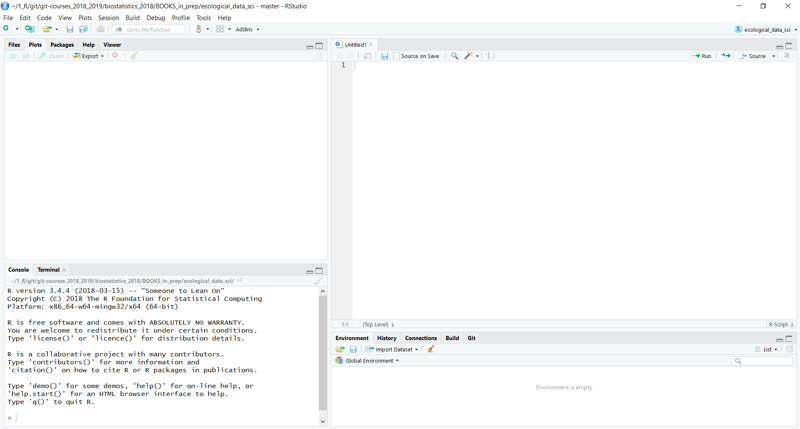
\includegraphics[width=11.11in]{/Users/nlb24/OneDrive - University of Pittsburgh/0-books/compbio4all_bk/compbio4all-book/images/RStudio_1st_view-800x600} \caption{RStudio when first opened.}(\#fig:rstudio.open)
\end{figure}

When referring to RStudio (and equivalently RSTudio Cloud - this is the last time I'll mention this so hopefully get get the point), there are two terms that need to be understood. As shown in Figure 3, there is 1)the \textbf{console} section of RStudio and 2) the \textbf{script editor} or \textbf{source viewer}.

\begin{figure}
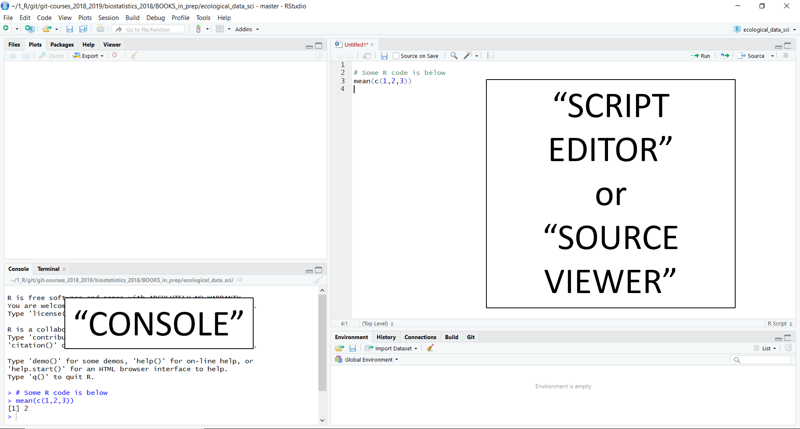
\includegraphics[width=11.11in]{/Users/nlb24/OneDrive - University of Pittsburgh/0-books/compbio4all_bk/compbio4all-book/images/RStudio_console_vs_script_editor-800x600} \caption{RStudio's console and script editor.}(\#fig:rstudio.console)
\end{figure}

(A ``cheat sheet'' called the ``RStudio IDE Cheat Sheet'' details all of RStudio's many features and is available at \url{https://www.rstudio.com/resources/cheatsheets/} . It very thorough, though a bit dense. I don't recommend it for beginners but you should remember that it exists.)

\hypertarget{the-console-versus-the-script-editor}{%
\subsection{The console versus the script editor}\label{the-console-versus-the-script-editor}}

You can type and enter text into both the \textbf{console} and the \textbf{script editor} (also called the \textbf{source viewer}. The console, however, responds actively like a calculator, while the script editor works more like a text editor. Information can be passes unidirectionally from the script editor to the console, but not the other way.

\hypertarget{the-r-console}{%
\subsubsection{The R console}\label{the-r-console}}

The \textbf{console} in RStudio gives you \textbf{interactive programming} environment that is very similar to a scientific calculator. If you click your mouse inside the console and type \texttt{1\ +\ 1} then press enter you will see the following type of output

\begin{Shaded}
\begin{Highlighting}[]
\DecValTok{1} \SpecialCharTok{+} \DecValTok{1}
\end{Highlighting}
\end{Shaded}

\begin{verbatim}
## [1] 2
\end{verbatim}

Note that right in front of where you typed \texttt{1+1} there is a \texttt{\textgreater{}} symbol. This is always in the R console and never needs to be typed. You may occasionally see it printed in books or on websites, but it doesn't ever need to be typed.

One thing to note about R is that it's not particular about spacing. All of the following things will yield the same results

\begin{Shaded}
\begin{Highlighting}[]
\DecValTok{1}\SpecialCharTok{+}\DecValTok{1}
\DecValTok{1} \SpecialCharTok{+} \DecValTok{1}
\DecValTok{1}          \SpecialCharTok{+}        \DecValTok{1}
\DecValTok{1} \SpecialCharTok{+}                                   \DecValTok{1}
\end{Highlighting}
\end{Shaded}

Got it? Awesome! Now we're ready for some real data analysis.

\hypertarget{book-getting-started-with-r}{%
\chapter*{(BOOK) Getting started with R}\label{book-getting-started-with-r}}
\addcontentsline{toc}{chapter}{(BOOK) Getting started with R}

\hypertarget{section}{%
\subsection*{}\label{section}}
\addcontentsline{toc}{subsection}{}

\textbf{NEW text}

In Book 2 we'll get started using R. We'll focus on jumping in with some simple examples that tell interesting scientific stories so we can get a sense for the power of R. Later, we'll dig deeper - bit by bit - not the details. Like any language R is a versatile tool for communication, but has conventions, quirks, idioms and dialects that new users have to become comfortable with. In general my goal in Book 2 will be to help you get a general sense of R, let you see a bit of the wild -- and overwhelming -- world of possibilities for how R is written, and outline the more specific aspects I'll use to help facilitate learning.

We'll have three specific goals:

\begin{enumerate}
\def\labelenumi{\arabic{enumi}.}
\tightlist
\item
  Run some initial, simple commands in R to see how it works.
\item
  Take a broad tour of the wide world of R so see the many faces of R code you may encounter in the wild.
\item
  Highlight the particular way coding conventions and idioms of R I'll use.
\item
  Introduce briefly some of the different ways you can get data into R.
\end{enumerate}

If you find yourself getting confused or overwhelmed don't panic A goal of this section is to prevent \emph{future} confusion by giving you a sense for the many different ways R can be written and that you will eventually encounter on the internet or other books, and to contrast them with what you'll use in this book. Here, I've worked to keep things consistent and to either use the simplest methods to accomplish the goal or to carefully break down hard tasks or concepts so you can master them. Once you start typing into your search engine ``R code \ldots{}'' you will get MANY different types of code which you may not yet be prepared to work with.

\hypertarget{hello-r-a-first-encounter-with-data-visualization}{%
\chapter{Hello R! A first encounter with data visualization}\label{hello-r-a-first-encounter-with-data-visualization}}

\hypertarget{key-ideas}{%
\section{Key Ideas}\label{key-ideas}}

\begin{itemize}
\tightlist
\item
  \textbf{Commands}: R uses simple typed commands to do \emph{everything.}
\item
  \textbf{Data}: loading data that comes with R using the \texttt{data()} command.
\item
  \textbf{Plotting}: Making simple plots with the \texttt{plot()} command.
\end{itemize}

\hypertarget{data-in-r}{%
\section{Data in R}\label{data-in-r}}

We'll start our exploration of R with a classic dataset from ecology and statistics showing one of the most striking patterns in wildlife biology: (\textbf{population cycles}){[}\url{https://en.wikipedia.org/wiki/Population_cycle}{]}. Populations are always changing, whether it is declines in the number bacteria in our gut after we take an antibiotic or increases in
raptor species after highly toxic pesticides were banned in the mid-twentieth century.

\begin{figure}
\centering
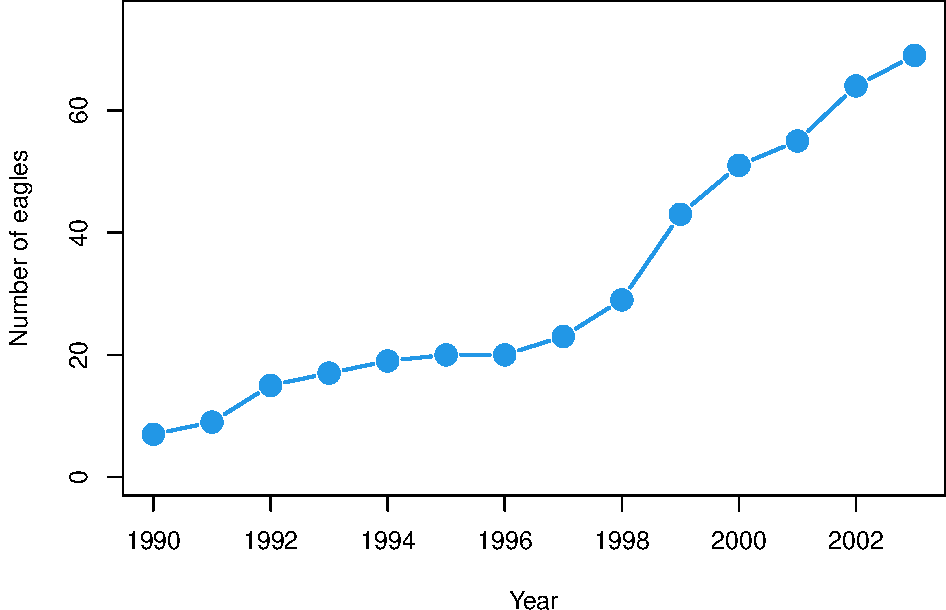
\includegraphics{compbio4all-book_files/figure-latex/unnamed-chunk-3-1.pdf}
\caption{\label{fig:unnamed-chunk-3}Growth of Eagle population in Pennsylvania, USA}
\end{figure}

In stark contrast, a few unique animals populations show dramatic \textbf{oscillations}, with rapid increases soon followed by dramatic drops, as if the population were on a roller coaster. One such population are Canada lynx (\emph{Lynx canadensis}) in Canada.

Lynx are (unfortunately) prized for their soft fur. In years when there are many lynx, trappers kill many lynx; in years when there are few lynx, trappers kill few (however, the number of lynx killed by humans does not contribute to the cycle). Records from fur industry have been compiled by ecologists for over a century to investigate what drives changes in lynx numbers. The table below shows a snapshot of these data, starting from the earliest available records in 1821.

\begin{longtable}[]{@{}
  >{\centering\arraybackslash}p{(\columnwidth - 2\tabcolsep) * \real{0.10}}
  >{\centering\arraybackslash}p{(\columnwidth - 2\tabcolsep) * \real{0.25}}@{}}
\caption{Number of lynx trapped in Canada}\tabularnewline
\toprule
\begin{minipage}[b]{\linewidth}\centering
year
\end{minipage} & \begin{minipage}[b]{\linewidth}\centering
lnyx.population
\end{minipage} \\
\midrule
\endfirsthead
\toprule
\begin{minipage}[b]{\linewidth}\centering
year
\end{minipage} & \begin{minipage}[b]{\linewidth}\centering
lnyx.population
\end{minipage} \\
\midrule
\endhead
1821 & 269 \\
1822 & 321 \\
1823 & 585 \\
1824 & 871 \\
1825 & 1475 \\
1826 & 2821 \\
1827 & 3928 \\
1828 & 5943 \\
1829 & 4950 \\
1830 & 2577 \\
1831 & 523 \\
1832 & 98 \\
1833 & 184 \\
1834 & 279 \\
1835 & 409 \\
\bottomrule
\end{longtable}

You've probably plotted data like this by hand using graph paper, point by point by locating the x-y coordinates. When plotting data like this, time (in this case ``year'') goes on the horizontal \textbf{x-axis}, and the changing variable (lynx.population) goes on the vertical \textbf{y-axis}. In a \textbf{spreadsheet}, you could highlight these columns and click on the ``Make graph'' icons to make the initial plot, then adjust things by clicking on parts of the plot you want to change.

Spreadsheets are said to operate under the principle of \textbf{``What You See Is What You Get''}, or \textbf{WYSIYGY}. They use a fully mouse-drive \textbf{Graphical User Interface (GUI)} where everything is done by pointing and clicking. Every time you make a plot you do these steps.

R is \emph{very} different - you only see things when you want to see them and you do everything via typed commands. This is a large paradigm shift for most people, so we'll start very very slow.

\hypertarget{loading-data-that-comes-with-r}{%
\section{Loading data that comes with R}\label{loading-data-that-comes-with-r}}

The Canada lynx is not just famous with ecologists but also familiar to statisticians who have frequently used it to test statistical methods for studying \textbf{time series} - basically long-term datasets of the same thing. Because of this, these lynx data are embedded within R and easy to access: all you have to do is type \texttt{data(lynx)} into the console and press the ``Enter'' key.

\begin{Shaded}
\begin{Highlighting}[]
\FunctionTok{data}\NormalTok{(lynx)}
\end{Highlighting}
\end{Shaded}

You might be wondering ``\emph{Ok, now what?}'' because nothing apparently happened. What you've done, though is loaded the \texttt{lynx} data into R's active memory, where it will wait for you next command.

Loading your own data into programs such as R can be a pain, so I'll use techniques such as use the \texttt{data()} command to make things as smooth as possible. I'll also introduce other methods, such as loading small datasets using code and downloading them from the internet. I'll also provide a thorough overview in the Appendices.

\hypertarget{plotting-simple-datasets-with-plot}{%
\section{\texorpdfstring{Plotting simple datasets with \texttt{plot()}}{Plotting simple datasets with plot()}}\label{plotting-simple-datasets-with-plot}}

Now in the console type \texttt{plot(lynx)} and press enter. You should see readout like what you see below \ldots{}

\begin{Shaded}
\begin{Highlighting}[]
\FunctionTok{plot}\NormalTok{(lynx)}
\end{Highlighting}
\end{Shaded}

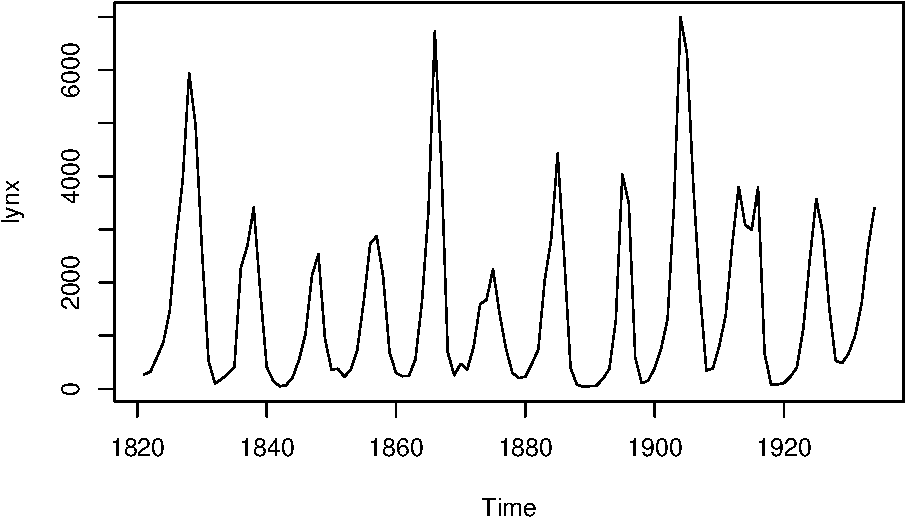
\includegraphics{compbio4all-book_files/figure-latex/unnamed-chunk-6-1.pdf}

\ldots{} and this intriguing plot. The x-axis is time from the early 1800s to the early 1900s, and the y-axis is the number of lynx pelts. This pattern continues to today, and it causes have kept ecologists working hard for over 100 years. Moreover, statistical analyses of data such as these have similarly kept statisticians busy.

This is a simplified example, but that's the basics of working in R:

\begin{enumerate}
\def\labelenumi{\arabic{enumi}.}
\tightlist
\item
  Load data
\item
  Use commands like \texttt{plot} tell R to do something with.
\end{enumerate}

For most of this book we'll use data that's been mostly pre-packaged for you to work with and loaded using the \texttt{data()} command. Real data analyses require more steps, and later in the book we'll briefly cover them so you are familiar with them when you see them elsewhere; further details can also be found in the Appendix.

\hypertarget{commands-in-r}{%
\section{Commands in R}\label{commands-in-r}}

The words ``data'' and ``plot'' in R represent \textbf{commands}; R associates specific code and therefore actions with these words To indicate commands in the text I'll always write it like this: \texttt{data()}. The parentheses are very important in R; forget one of them, and things won't work. After the word representing the command there is always a \textbf{parenthesis} \texttt{(}. Other things such as the name of a dataset go after the first parenthesis, and the command is completed with a matching parenthesis \texttt{)}. To emphasis that things using go within the parentheses I will often write commands like this \texttt{data(...)}, where the \texttt{...} in this case is the name of a dataset.

In some cases you can issue a command, like \texttt{data()}, and R does something only behind the scenes. Often, though, we'll elicit a reaction from R, either data will appear in the Console or a plot will be created.

\hypertarget{the-structure-of-commands-in-r}{%
\section{The structure of commands in R}\label{the-structure-of-commands-in-r}}

Our use of the \texttt{plot()} command was pretty standard; there were two pieces to it:

\begin{enumerate}
\def\labelenumi{\arabic{enumi}.}
\tightlist
\item
  The command, \texttt{plot()}
\item
  The data, \texttt{lynx}
\end{enumerate}

Data in R -- and especially in computational biology -- can take on many forms, which we'll cover as needed as throughout the book. All data is presented in R by an \textbf{object} stored behind the scenes in R's memory. The fact that data in R is usually resting out of view until we do something explicitly with it can take some getting used to, since usually we work with data printed out on a page or displayed in a spreadsheet.

Commands in R almost always include an object within them. Next we'll consider something else that go with commands : \textbf{arguments}.

\hypertarget{arguements-in-r}{%
\section{Arguements in R}\label{arguements-in-r}}

A common mathematical operation when doing data analysis is taking the \textbf{log} of something. (For now we won't worry about what the log is or why we use it' we'll come back to this little bit of math frequently though). We can tell R to plot the log of our lynx data by adding the argument \texttt{log\ =\ "y"} to the \texttt{plot(...)} command. This alters the graph a bit which, for some particular data analysis purposes, will come in handy (more on that later).

\begin{Shaded}
\begin{Highlighting}[]
\FunctionTok{plot}\NormalTok{(lynx, }\AttributeTok{log =} \StringTok{"y"}\NormalTok{)}
\end{Highlighting}
\end{Shaded}

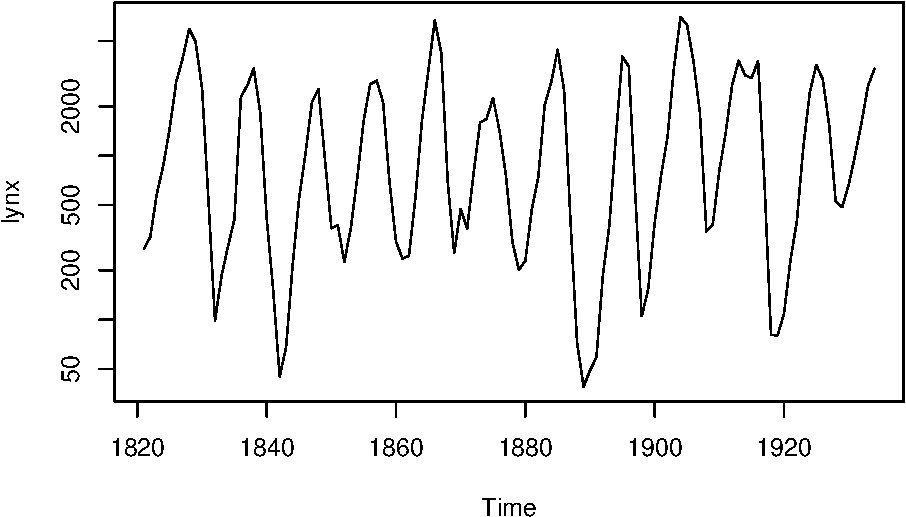
\includegraphics{compbio4all-book_files/figure-latex/unnamed-chunk-7-1.pdf}

In the code above \texttt{log} is the argument and \texttt{"y"} is the \textbf{value} assigned to the argument.

Arguments \textbf{always} have an equals sign with them, so I'll emphasize this by typically writing them as \texttt{argument.name\ =\ ...}. One tricky thing about arguments is that they can take on letters, words, or numbers, and sometimes there need to be quotation marks like \texttt{log\ =\ "y"}, but not always.

Since arguments are fairly tricky, they are a common source of errors, such as forgetting \texttt{=}, or putting the value of the argument in the wrong format.

\hypertarget{arguements-and-more-arguments}{%
\section{Arguements and more arguments}\label{arguements-and-more-arguments}}

We now have three things going on

\begin{enumerate}
\def\labelenumi{\arabic{enumi}.}
\tightlist
\item
  A \textbf{command}, \texttt{plot()}
\item
  A \textbf{data object}, \texttt{lynx}
\item
  An \textbf{argument}, \texttt{log\ =\ "y"}
\end{enumerate}

Most functions in R have multiple arguments that can be invoked Try the following code \texttt{plot(lynx,\ col\ =\ 3)}. That is the \texttt{plot()} function with the argument \texttt{col\ =\ 3} added. What do you think \texttt{col\ =\ 2} means? Try different values like 4, 5, and 6.

\begin{Shaded}
\begin{Highlighting}[]
\FunctionTok{plot}\NormalTok{(lynx, }\AttributeTok{col =} \DecValTok{2}\NormalTok{)}
\end{Highlighting}
\end{Shaded}

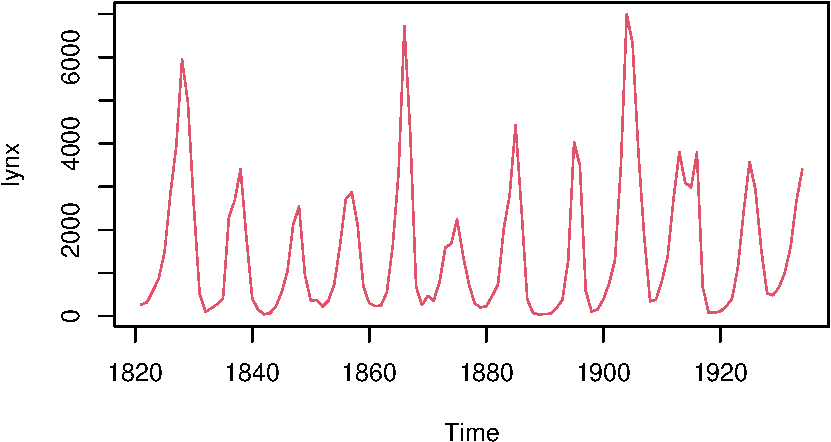
\includegraphics{compbio4all-book_files/figure-latex/unnamed-chunk-8-1.pdf}

Now try this: \texttt{plot(lynx,\ type\ =\ "p")}

Note that there are quotation marks around the p.

\begin{Shaded}
\begin{Highlighting}[]
\FunctionTok{plot}\NormalTok{(lynx, }\AttributeTok{type =} \StringTok{"p"}\NormalTok{)}
\end{Highlighting}
\end{Shaded}

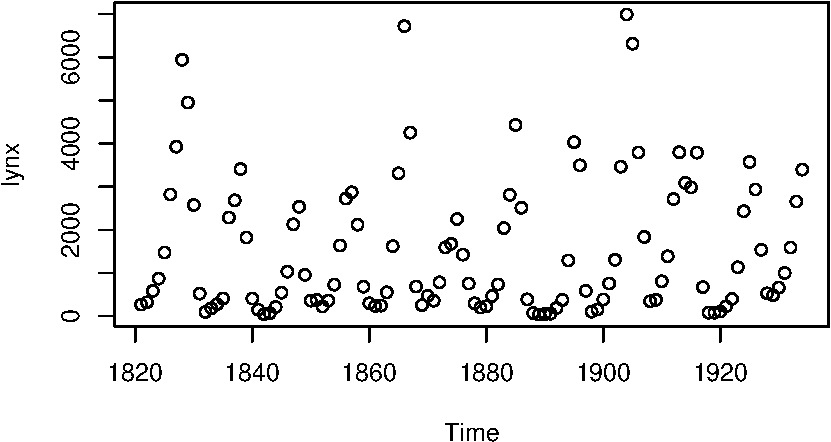
\includegraphics{compbio4all-book_files/figure-latex/unnamed-chunk-9-1.pdf}

Now instead of ``p'' use ``b'', which stands for ``both''. What do you think the ``both'' is referring to?

\begin{Shaded}
\begin{Highlighting}[]
\FunctionTok{plot}\NormalTok{(lynx, }\AttributeTok{type =} \StringTok{"b"}\NormalTok{)}
\end{Highlighting}
\end{Shaded}

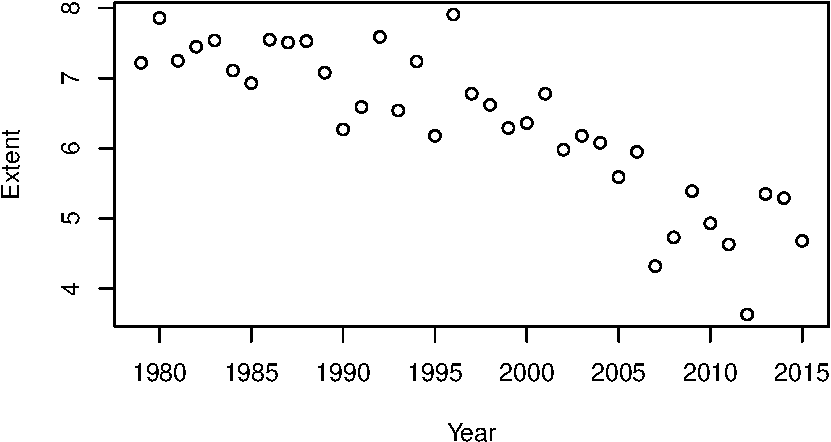
\includegraphics{compbio4all-book_files/figure-latex/unnamed-chunk-10-1.pdf}

\begin{Shaded}
\begin{Highlighting}[]
\DocumentationTok{\#\# }\AlertTok{TODO}\DocumentationTok{: add followup exercises}
\DocumentationTok{\#\#\# R, biology}
\DocumentationTok{\#\# }\AlertTok{TODO}\DocumentationTok{ Add as optional? cover elsewhere}

\FunctionTok{plot}\NormalTok{(}\FunctionTok{log}\NormalTok{(lynx))}
\end{Highlighting}
\end{Shaded}

\hypertarget{multiple-arguments-at-the-same-time}{%
\section{Multiple arguments at the same time}\label{multiple-arguments-at-the-same-time}}

Functions can not only have multiple arguments, but they can \textbf{take on} multiple arguments at the same time. Let's feed two arguments to \texttt{plot()}, \texttt{col\ =\ ...} and a new one, \texttt{type\ =\ ...}.

\begin{Shaded}
\begin{Highlighting}[]
\FunctionTok{plot}\NormalTok{(lynx, }\AttributeTok{col =} \DecValTok{4}\NormalTok{, }\AttributeTok{type =} \StringTok{"b"}\NormalTok{)}
\end{Highlighting}
\end{Shaded}

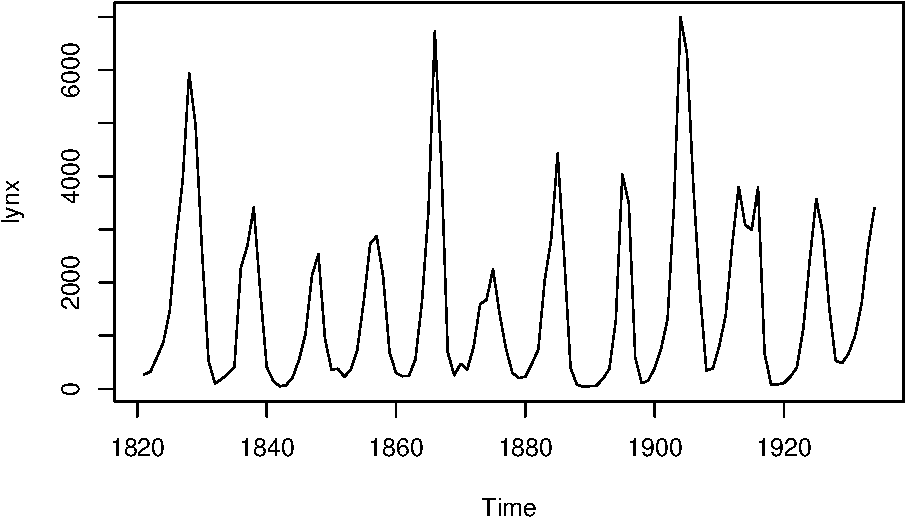
\includegraphics{compbio4all-book_files/figure-latex/unnamed-chunk-12-1.pdf}

Examine the series of plots below; what do you thing \texttt{type=...} is referring to?
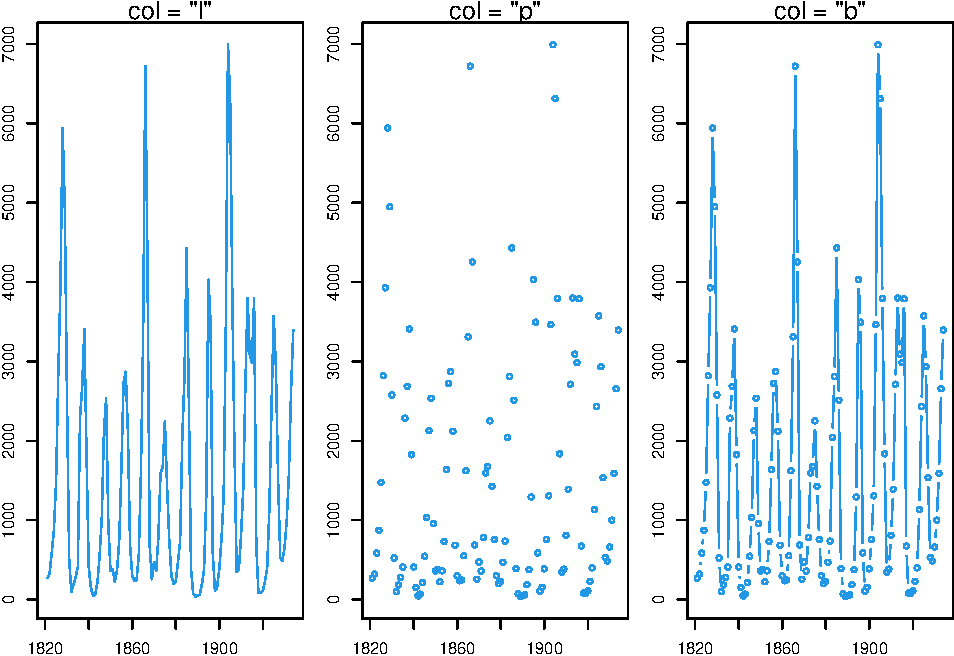
\includegraphics{compbio4all-book_files/figure-latex/unnamed-chunk-13-1.pdf}

\hypertarget{r-commands-and-line-breaks}{%
\section{R commands and line breaks}\label{r-commands-and-line-breaks}}

A cool thing about R is that it doesn't care about \textbf{line breaks} within a command, so I can do this if I want:

\begin{Shaded}
\begin{Highlighting}[]
\FunctionTok{plot}\NormalTok{(lynx, }
     \AttributeTok{col =} \DecValTok{4}\NormalTok{, }
     \AttributeTok{type =} \StringTok{"b"}\NormalTok{)}
\end{Highlighting}
\end{Shaded}

Or if for some reason this

\begin{Shaded}
\begin{Highlighting}[]
\FunctionTok{plot}\NormalTok{(lynx,  }\AttributeTok{col =} \DecValTok{4}\NormalTok{, }
     \AttributeTok{type =} \StringTok{"b"}\NormalTok{)}
\end{Highlighting}
\end{Shaded}

Or even this

\begin{Shaded}
\begin{Highlighting}[]
\FunctionTok{plot}\NormalTok{(lynx,  }
     
     \AttributeTok{col =} \DecValTok{4}\NormalTok{, }
     
     
     \AttributeTok{type =} \StringTok{"b"}\NormalTok{)}
\end{Highlighting}
\end{Shaded}

\hypertarget{code-comments}{%
\section{Code comments}\label{code-comments}}

One thing that putting thing on multiple lines allows you do to is add \textbf{comments} to your code if you place a hashtag (aka pound symbol) in front of it.

\begin{Shaded}
\begin{Highlighting}[]
\FunctionTok{plot}\NormalTok{(lynx,          }\CommentTok{\# data object}
     \AttributeTok{col =} \DecValTok{4}\NormalTok{,       }\CommentTok{\# color argument}
     \AttributeTok{type =} \StringTok{"b"}\NormalTok{)  }\CommentTok{\# type of graph argument}
\end{Highlighting}
\end{Shaded}

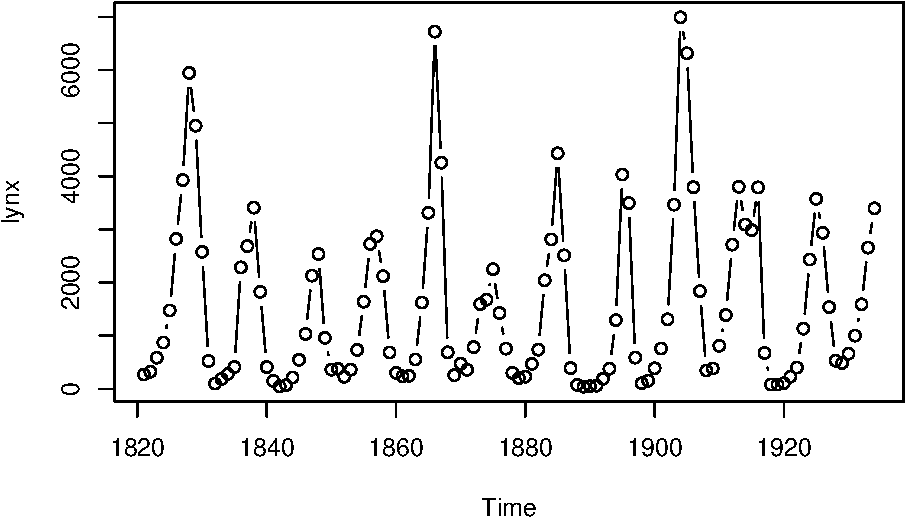
\includegraphics{compbio4all-book_files/figure-latex/unnamed-chunk-17-1.pdf}

\hypertarget{a-note-on-plotting}{%
\section{A note on plotting}\label{a-note-on-plotting}}

One of the great things about R is that it can make really nice plots. You'll soon see that there are many ways to do the same basic thing in R, and this includes making plot. \textbf{Data visualization} is a key aspect of modern science, so its important to build up your skills, including knowing about the different ways plots are made in R. Don't worry though - we'll build all of this up step by step.

\hypertarget{now-you-try-it}{%
\section{Now you try it}\label{now-you-try-it}}

\hypertarget{easy-tasks}{%
\subsection{Easy tasks}\label{easy-tasks}}

Fix each line of code below so the work

\begin{Shaded}
\begin{Highlighting}[]
\NormalTok{plot lynx}
\FunctionTok{plot}\NormalTok{(lynx}
\end{Highlighting}
\end{Shaded}

Examine the plots below. What does \texttt{pch\ =\ ...} do to the plot?
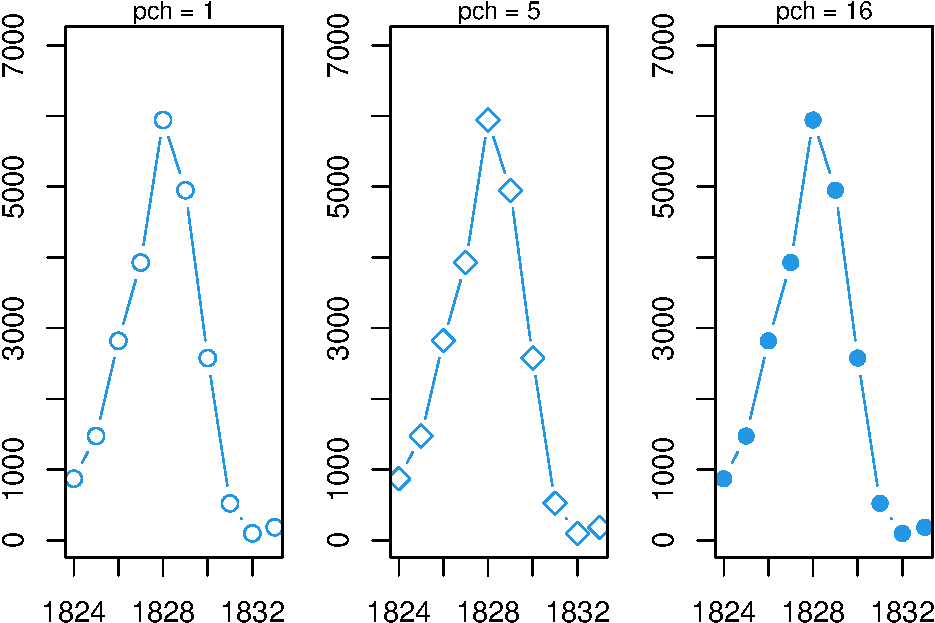
\includegraphics{compbio4all-book_files/figure-latex/unnamed-chunk-20-1.pdf}

Examine the plots below. What does \texttt{lwd\ =\ ...} do to the plot?
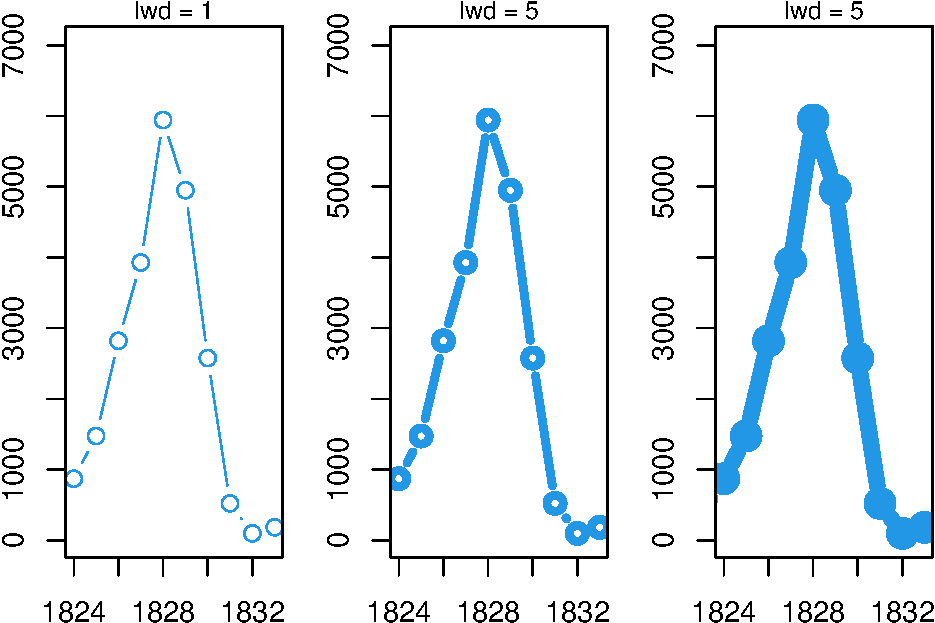
\includegraphics{compbio4all-book_files/figure-latex/unnamed-chunk-21-1.pdf}

Fix each argument below so the code works.

\begin{Shaded}
\begin{Highlighting}[]
\FunctionTok{plot}\NormalTok{(lynx, col  }\DecValTok{1}\NormalTok{)}
\FunctionTok{plot}\NormalTok{(lynx, }\AttributeTok{col =} \StringTok{"1"}\NormalTok{)}
\FunctionTok{plot}\NormalTok{(lynx, type b)}
\FunctionTok{plot}\NormalTok{(lynx, }\AttributeTok{type =}\NormalTok{ b)}
\FunctionTok{plot}\NormalTok{(lynx, type }\StringTok{"b"}\NormalTok{)}
\FunctionTok{plot}\NormalTok{(lynx type }\StringTok{"b"}\NormalTok{)}
\FunctionTok{plot}\NormalTok{(lynx, }\AttributeTok{type =}  \StringTok{"b)}
\end{Highlighting}
\end{Shaded}

\begin{Shaded}
\begin{Highlighting}[]
\FunctionTok{plot}\NormalTok{(lynx, col  }\DecValTok{1}\NormalTok{, }\AttributeTok{type =} \StringTok{"b)}
\StringTok{plot(lynx, col = "}\DecValTok{1}\StringTok{", type = b)}
\StringTok{plot(lynx, pch = 1, type b)}
\StringTok{plot(lynx, pch 1 type = b)}
\StringTok{plot(lynx, lwd = "}\DecValTok{2}\StringTok{" type "}\NormalTok{b}\StringTok{")}
\StringTok{plot(lynx pch = 2, type "}\NormalTok{b}\StringTok{")}
\StringTok{plot(lynx, lwd = 3 type =  "}\NormalTok{b)}
\end{Highlighting}
\end{Shaded}

Split the following code between multiple lines and add a comment between each of them to indicate what the argument does.

\begin{Shaded}
\begin{Highlighting}[]
\FunctionTok{plot}\NormalTok{(lynx, }\AttributeTok{type =} \StringTok{"b"}\NormalTok{, }\AttributeTok{pch =}  \DecValTok{2}\NormalTok{,)}
\end{Highlighting}
\end{Shaded}

\hypertarget{intermediate-tasks}{%
\subsection{Intermediate tasks}\label{intermediate-tasks}}

Here's a challenge: there is another dataset that comes with R called \texttt{sunspot.year} There was once a hypothesized link between the Canada lynx and sunspots that we'll explore later; right now we'll just check it out. See if you can do the following things on your own in the R console.

\hypertarget{make-a-simple-plot}{%
\subsubsection*{Make a simple plot}\label{make-a-simple-plot}}
\addcontentsline{toc}{subsubsection}{Make a simple plot}

\begin{enumerate}
\def\labelenumi{\arabic{enumi}.}
\tightlist
\item
  Using the \texttt{data()} command, load \texttt{sunspot.year} data into R's active memory
\item
  Plot the data.
\end{enumerate}

Your plot should look like this:

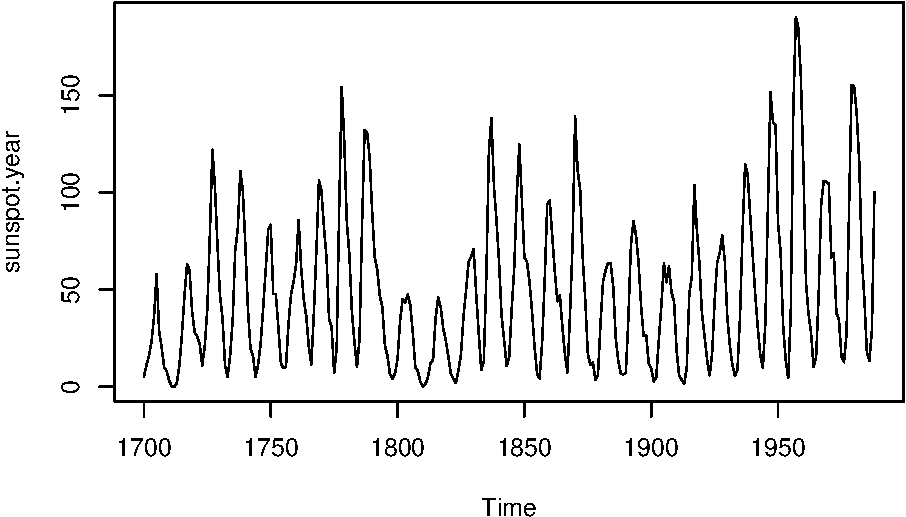
\includegraphics{compbio4all-book_files/figure-latex/unnamed-chunk-27-1.pdf}

\hypertarget{modify-your-plot}{%
\subsubsection*{Modify your plot}\label{modify-your-plot}}
\addcontentsline{toc}{subsubsection}{Modify your plot}

\begin{enumerate}
\def\labelenumi{\arabic{enumi}.}
\tightlist
\item
  Use the \texttt{col\ =} argument to make the color of the line different than black.
\item
  Use the \texttt{type\ =} argument to make the plot show points connected by a line.
\end{enumerate}

Your plot should look like this:

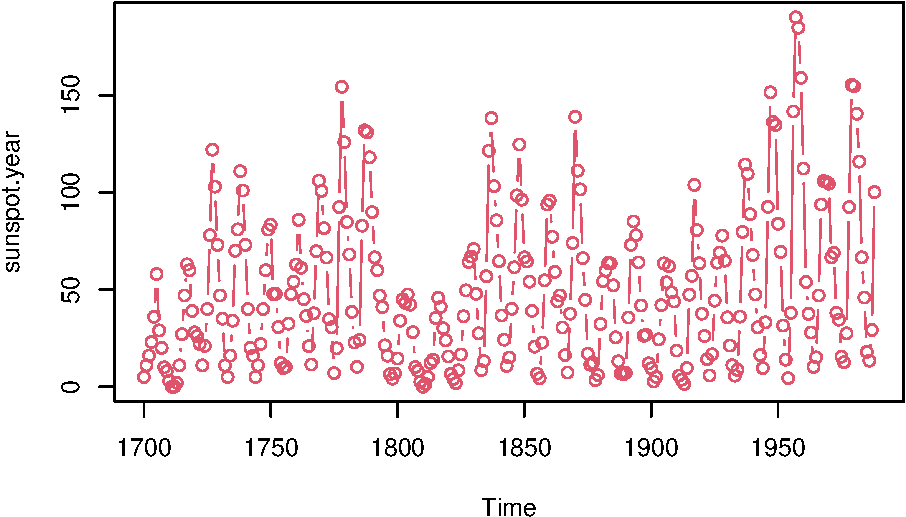
\includegraphics{compbio4all-book_files/figure-latex/unnamed-chunk-28-1.pdf}

\hypertarget{plot-on-the-log-scale}{%
\subsubsection*{Plot on the log scale}\label{plot-on-the-log-scale}}
\addcontentsline{toc}{subsubsection}{Plot on the log scale}

Plot the sunspot data on the log scale. Note: you will get a warnig in red text - you can ignore this.

\begin{verbatim}
## Warning in xy.coords(x, NULL, log = log, setLab = FALSE): 3 y values <= 0
## omitted from logarithmic plot
\end{verbatim}

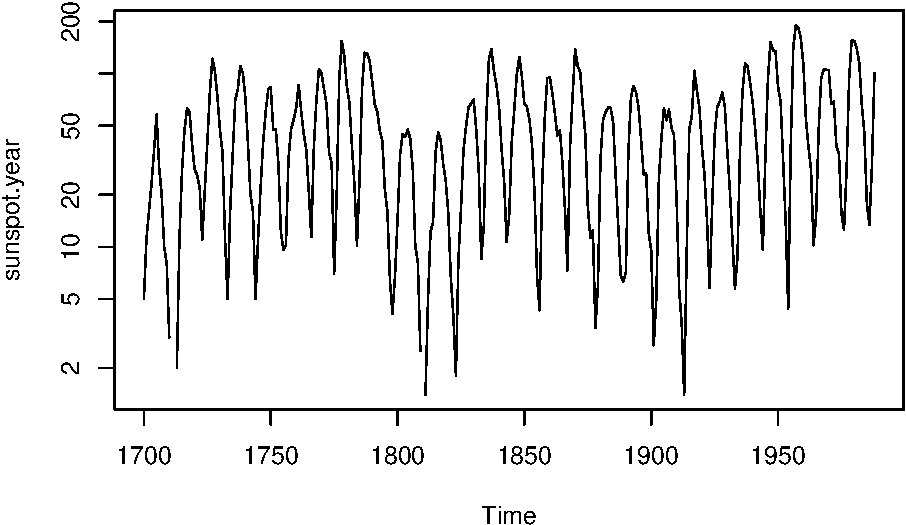
\includegraphics{compbio4all-book_files/figure-latex/unnamed-chunk-29-1.pdf}

\hypertarget{downloading-r-packages-and-their-data}{%
\chapter{Downloading R packages (and their data)}\label{downloading-r-packages-and-their-data}}

In the previous chapter we used some data the comes with R. In this lesson we'll start expanding out from the \textbf{Base R distribution} and exploring the ways that external \textbf{packages} extend R.

\hypertarget{loading-data-from-r-packages}{%
\section{Loading data from R packages}\label{loading-data-from-r-packages}}

\textbf{NEW text:}
When you install R you get *Base R**, which is the core set of functions, functionality, and some data sets. Base R is surrounded by a universe of extensions built by statistician, programmers, academics and businesses that use R for analyses. A lot of R's functionality is found in these packages, including data sets, special plotting functions, and statistical tools for the analysis of complex data. These have to be downloaded from the internet and installed. Most packages contain data in order to demonstrate what they do.

Most R packages you'll use are stored on the CRAN website where you download R (\url{https://cran.r-project.org/}). R and RStudio have functions and tools for downloading and managing packages that we'll briefly introduce in this exercise.

Another major platform for packages is called \textbf{Bioconductor}; we'll cover downloading packages from there later. Finally, many packages are hosted on a site called \textbf{GitHub}. This book relies heavily on an R package I've written and hosted on GitHub called \texttt{combio4all} (\url{https://brouwern.github.io/compbio4all/}) that contains the datasets used throughout the book, as well as some helpful R functions I've written. Many packages on CRAN also occur on GitHub, especially if programmers are actively developing, updating, and managing the package. We'll cover downloading packages from GitHub later.

\hypertarget{functions-arguements}{%
\subsection{Functions \& Arguements}\label{functions-arguements}}

\begin{itemize}
\tightlist
\item
  \texttt{install.packages()}

  \begin{itemize}
  \tightlist
  \item
    Argument: \texttt{dependencies\ =\ TRUE}
  \end{itemize}
\item
  \texttt{library()}
\end{itemize}

\begin{center}\rule{0.5\linewidth}{0.5pt}\end{center}

\hypertarget{optional-what-functions-come-with-base-r}{%
\section{OPTIONAL: What functions come with base R?}\label{optional-what-functions-come-with-base-r}}

\textbf{The following section is OPTIONAL}

If for some reason you want to see \emph{all} the functions that come with the distribution base R, type this into the console and press enter. (\texttt{ls} stands for ``list'' and is a function we'll use more later).

\begin{Shaded}
\begin{Highlighting}[]
\CommentTok{\# this code chunk is OPTIONAL}
\FunctionTok{ls}\NormalTok{(}\StringTok{"package:base"}\NormalTok{)}
\end{Highlighting}
\end{Shaded}

As R has been developed there has also built up a cannon of tried and true packages that are downloaded automatically when you download R. If you want to see all of the packages that come with base R, do this. \texttt{library()} is a function you will use a lot.

\begin{Shaded}
\begin{Highlighting}[]
\CommentTok{\# this code chunk is OPTIONAL}
\FunctionTok{.libPaths}\NormalTok{(}\StringTok{""}\NormalTok{) }
\FunctionTok{library}\NormalTok{()}
\end{Highlighting}
\end{Shaded}

One package that is part of this cannon is \texttt{MASS}, which stands for Modern Applied Statistics in S. ``S'' is the precursor to R, and MASS is the package that accompanies the book of the same name, which is one of the original books on S/R. (\url{https://www.springer.com/us/book/9780387954578})

\textbf{End OPTIONAL section}

\begin{center}\rule{0.5\linewidth}{0.5pt}\end{center}

\hypertarget{load-data-from-an-external-r-package}{%
\section{Load data from an external R package}\label{load-data-from-an-external-r-package}}

Many packages have to be explicitly downloaded and installed in order to use their functions and datasets. Note that this is a \textbf{two-step process}:

\begin{enumerate}
\def\labelenumi{\arabic{enumi}.}
\tightlist
\item
  Download package from internet with \texttt{install.packages(...)}
\item
  Explicitly tell R to load it with \texttt{library(...)}
\end{enumerate}

\hypertarget{step-1-downloading-packages-install.packages...}{%
\subsection{\texorpdfstring{Step 1: Downloading packages \texttt{install.packages(...)}}{Step 1: Downloading packages install.packages(...)}}\label{step-1-downloading-packages-install.packages...}}

There are a number of ways to install packages. One of the easiest is to use the function \texttt{install.packages()}. Note that it might be better to call this ``download.packages'' since after you download it, you still have to load it! (Lots of confusion has resulted from calling this function ``install.packages'').

We'll download a package with lots of interesting biology data called \texttt{Stat2Data}. Note that in the \textbf{call} to \texttt{install.packages(...)}, the name of the package is in quotes.

\begin{Shaded}
\begin{Highlighting}[]
\FunctionTok{install.packages}\NormalTok{(}\StringTok{"Stat2Data"}\NormalTok{)}
\end{Highlighting}
\end{Shaded}

Often when you download a package you'll see a fair bit of red text. Usually there's nothing of interest here, but sometimes you need to read over it for hints about why something didn't work.

For example, when I downloaded this package I got this cryptic message in bright red text:
\texttt{trying\ URL\ \textquotesingle{}https://cran.rstudio.com/bin/macosx/contrib/4.0/Stat2Data\_2.0.0.tgz\textquotesingle{}}
\texttt{Content\ type\ \textquotesingle{}application/x-gzip\textquotesingle{}\ length\ 1177728\ bytes\ (1.1\ MB)}
\texttt{==================================================}
\texttt{downloaded\ 1.1\ MB}

Followed by this in less insistent black:
\texttt{The\ downloaded\ binary\ packages\ are\ in}
\texttt{/var/folders/q8/gwjfr69n05vf4h15l6hdl4d8x1zk5v/T//RtmpeRHx2y/downloaded\_packages}

This is all perfectly normal, so don't worry.

\hypertarget{protip-dont-re-download-packages-all-the-time}{%
\subsubsection{Protip: don't re-download packages all the time}\label{protip-dont-re-download-packages-all-the-time}}

You can think of R and RStudio like a computer operating systems, and packages like software you chose to download. R, RStudio and packages will need to be updated at times - indeed, the first step in diagnosing many problems with R is to update things. But updates probably only need to be done every six months or so at the most; I generally wait until things stop working.

Anytime a lesson introduces a new package I'll include code to do the download. You only need to do this once unless you start encountering a problems. A way to make this happen is to \textbf{comment out} the code by putting a hashtag in front of it like this

\begin{Shaded}
\begin{Highlighting}[]
\CommentTok{\# install.packages("Stat2Data")}
\end{Highlighting}
\end{Shaded}

This preserves the code but tells R \emph{``don't run this line.''}

\hypertarget{step-2-explicitly-loading-a-package}{%
\subsection{Step 2: Explicitly loading a package}\label{step-2-explicitly-loading-a-package}}

The \texttt{install.packages()} function just downloads the package software to R; now you need to tell R explicitly \emph{``I want to work with the package''}. This is done using the \texttt{library()} function. (Its called library because another name for packages is \textbf{libraries}. ).

\begin{Shaded}
\begin{Highlighting}[]
\FunctionTok{library}\NormalTok{(Stat2Data)}
\end{Highlighting}
\end{Shaded}

As frequently is the case, R doesn't look like its doing much, but you've actually just installed a bunch of cool datasets.

In contrast to running \texttt{install.packages()}, \texttt{library()} need to be run \textbf{every time you use the code}. More specifically, every time you re-start R. What happens is when you shut down R, all the packages you loaded using \texttt{library()} are taken out of memory. Next time you use R you need to re-load them using \texttt{libary()}.

\begin{center}\rule{0.5\linewidth}{0.5pt}\end{center}

\hypertarget{optional-seeing-all-of-your-installed-packages}{%
\section{OPTIONAL: Seeing all of your installed packages}\label{optional-seeing-all-of-your-installed-packages}}

\textbf{The following section is OPTIONAL}

If for some reason you want to see everything you've downloaded, do this.

\begin{Shaded}
\begin{Highlighting}[]
\CommentTok{\# This code is optional}
\FunctionTok{installed.packages}\NormalTok{()}
\end{Highlighting}
\end{Shaded}

\textbf{End OPTIONAL section}

\begin{center}\rule{0.5\linewidth}{0.5pt}\end{center}

\hypertarget{downloading-packages-using-rstudio}{%
\section{Downloading packages using RStudio}\label{downloading-packages-using-rstudio}}

RStudio has a point-and-click interface to download packages. In the pane of the RStudio GUI that says ``Files, Plots, Packages, Help, Viewer'' click on ``Packages''. Below ``Packages'' it will then say ``Install, Update, ..,'' Click on ``Install.'' (There might be a lag during this process as RStudio gets info about your packages). In the pop up widow there will be a middle field ``Packages'' where you can type the name of the package you need. There's an auto-complete feature to help you in case you forget the name. Then click ``install.'' Note that in the bottom right corner of the pop up is a checked box next to ``Install dependencies.'' Leave that checked; more on that later.

This is a useful function, but I don't do this very often because I include any download information in my scripts.

\hypertarget{your-turn}{%
\section{Your turn}\label{your-turn}}

Fix this code

\begin{Shaded}
\begin{Highlighting}[]
\FunctionTok{install.packages}\NormalTok{(MASS)}
\FunctionTok{install.packages}\NormalTok{(}\StringTok{"car)}
\StringTok{install.packages ggplot2 }
\StringTok{install.packages(cowplot }
\StringTok{install.packagesggpubr }
\end{Highlighting}
\end{Shaded}

The package \texttt{carData} contains a time series dataset called USpop. Fix the following code to download and plot these data.

\begin{Shaded}
\begin{Highlighting}[]
\FunctionTok{install.packages}\NormalTok{(}\StringTok{"carData"}\NormalTok{)}
\FunctionTok{plot}\NormalTok{(USPop)}
\end{Highlighting}
\end{Shaded}

The package \texttt{boot} contains a dataset called \texttt{ducks} on the behavior of crosses between two species of ducks: Mallards and Pintails. Fix the following code to download and plot these data.

\begin{Shaded}
\begin{Highlighting}[]
\FunctionTok{install.packages}\NormalTok{(}\StringTok{"boot"}\NormalTok{)}
\FunctionTok{library}\NormalTok{(boot)}
\FunctionTok{plot}\NormalTok{(ducks)}
\end{Highlighting}
\end{Shaded}

\hypertarget{data-in-dataframes}{%
\chapter{Data in dataframes}\label{data-in-dataframes}}

An interesting dataset in \texttt{Stat2Data} is \texttt{SeaIce}. Load it with the \texttt{data()} command.

\begin{Shaded}
\begin{Highlighting}[]
\FunctionTok{library}\NormalTok{(Stat2Data)}
\FunctionTok{data}\NormalTok{(SeaIce)}
\end{Highlighting}
\end{Shaded}

\texttt{SeaIce} shows 37 years of the area of frozen ice in the arctic, from 1979 to 1993. The \texttt{lynx} data we worked with previously was in a special format that you'll probably rarely encounter ever again. It was nice to use, however, because it required very little code to plot.\\
SeaIce, however, is a typical R data object in the form of a \textbf{dataframe}. Dataframes are fundamental units of analysis in R. Most of the data you will load into R and work within R will be in a dataframe. The have the same basic structure as a spreadsheet, but R keeps them hidden in memory and you have to use commands to explore them.

\hypertarget{looking-at-dataframes-with-view}{%
\section{\texorpdfstring{Looking at dataframes with \texttt{View()}}{Looking at dataframes with View()}}\label{looking-at-dataframes-with-view}}

To get a spreadsheet-like view of a dataframe you can use the \texttt{View} command

\begin{Shaded}
\begin{Highlighting}[]
\FunctionTok{View}\NormalTok{(SeaIce)}
\end{Highlighting}
\end{Shaded}

This will bring up the data in a spreadsheet like viewer as a new tab in the script editor, similar to this.

\begin{longtable}[]{@{}
  >{\centering\arraybackslash}p{(\columnwidth - 6\tabcolsep) * \real{0.10}}
  >{\centering\arraybackslash}p{(\columnwidth - 6\tabcolsep) * \real{0.12}}
  >{\centering\arraybackslash}p{(\columnwidth - 6\tabcolsep) * \real{0.10}}
  >{\centering\arraybackslash}p{(\columnwidth - 6\tabcolsep) * \real{0.10}}@{}}
\toprule
\begin{minipage}[b]{\linewidth}\centering
Year
\end{minipage} & \begin{minipage}[b]{\linewidth}\centering
Extent
\end{minipage} & \begin{minipage}[b]{\linewidth}\centering
Area
\end{minipage} & \begin{minipage}[b]{\linewidth}\centering
t
\end{minipage} \\
\midrule
\endhead
1979 & 7.22 & 4.54 & 1 \\
1980 & 7.86 & 4.83 & 2 \\
1981 & 7.25 & 4.38 & 3 \\
1982 & 7.45 & 4.38 & 4 \\
1983 & 7.54 & 4.64 & 5 \\
1984 & 7.11 & 4.04 & 6 \\
1985 & 6.93 & 4.18 & 7 \\
1986 & 7.55 & 4.67 & 8 \\
1987 & 7.51 & 5.61 & 9 \\
1988 & 7.53 & 5.32 & 10 \\
\bottomrule
\end{longtable}

⚠️ \textbf{Note:} Unlike a spreadsheet you cannot edit the data when is called up using \texttt{View()} ⚠️

Like a spreadsheet the data are organized in columns and rows. Each \textbf{column} represents a type of information:

\begin{itemize}
\tightlist
\item
  \texttt{Year}: when data were collected
\item
  \texttt{Extent}: the amount of area within the ice-bound region
\item
  \texttt{Area}: total area of ice, minus any non-ice area (land, melted water)
\item
  \texttt{t}: time point, from 1 (1979) to 15 (1993)
\end{itemize}

You can think of \texttt{Extent} as similar to the size of a country, and \texttt{Area} as the actual amount of land in a country minus any lakes.

Each row represents a different year of data; row 1 is the \texttt{Extent} and \texttt{Area} for 1979, row to is the \texttt{Extent} and \texttt{Area} for 1980 and so on.

\hypertarget{looking-at-dataframes-in-the-console}{%
\section{Looking at dataframes in the console}\label{looking-at-dataframes-in-the-console}}

Another common way to examine data is simply type the name of the data in the console and press enter. This prints it out; however, if its a large data frame this may take up a LOT of room. (I'll just show an exert here).

\begin{Shaded}
\begin{Highlighting}[]
\NormalTok{SeaIce}
\end{Highlighting}
\end{Shaded}

\begin{verbatim}
##    Year Extent Area  t
## 1  1979   7.22 4.54  1
## 2  1980   7.86 4.83  2
## 3  1981   7.25 4.38  3
## 4  1982   7.45 4.38  4
## 5  1983   7.54 4.64  5
## 6  1984   7.11 4.04  6
## 7  1985   6.93 4.18  7
## 8  1986   7.55 4.67  8
## 9  1987   7.51 5.61  9
## 10 1988   7.53 5.32 10
## 11 1989   7.08 4.83 11
## 12 1990   6.27 4.51 12
## 13 1991   6.59 4.47 13
## 14 1992   7.59 5.38 14
## 15 1993   6.54 4.53 15
\end{verbatim}

\hypertarget{examining-part-of-a-dataframe}{%
\section{Examining part of a dataframe}\label{examining-part-of-a-dataframe}}

Look at the top of the dataframe

\begin{Shaded}
\begin{Highlighting}[]
\FunctionTok{head}\NormalTok{(SeaIce)}
\end{Highlighting}
\end{Shaded}

\begin{verbatim}
##   Year Extent Area t
## 1 1979   7.22 4.54 1
## 2 1980   7.86 4.83 2
## 3 1981   7.25 4.38 3
## 4 1982   7.45 4.38 4
## 5 1983   7.54 4.64 5
## 6 1984   7.11 4.04 6
\end{verbatim}

Look at the bottom

\begin{Shaded}
\begin{Highlighting}[]
\FunctionTok{tail}\NormalTok{(SeaIce)}
\end{Highlighting}
\end{Shaded}

\begin{verbatim}
##    Year Extent Area  t
## 32 2010   4.93 3.29 32
## 33 2011   4.63 3.18 33
## 34 2012   3.63 2.37 34
## 35 2013   5.35 3.75 35
## 36 2014   5.29 3.70 36
## 37 2015   4.68 3.37 37
\end{verbatim}

\hypertarget{get-information-about-dataframes}{%
\section{Get information about dataframes}\label{get-information-about-dataframes}}

The following commands give you important information about a dataframe.

\begin{Shaded}
\begin{Highlighting}[]
\FunctionTok{is}\NormalTok{(SeaIce)}
\FunctionTok{dim}\NormalTok{(SeaIce)}
\FunctionTok{names}\NormalTok{(SeaIce)}
\FunctionTok{summary}\NormalTok{(SeaIce)}
\FunctionTok{summary}\NormalTok{(SeaIce}\SpecialCharTok{$}\NormalTok{Extent)}
\FunctionTok{mean}\NormalTok{(SeaIce}\SpecialCharTok{$}\NormalTok{Extent)}
\FunctionTok{min}\NormalTok{(SeaIce}\SpecialCharTok{$}\NormalTok{Extent)}
\FunctionTok{max}\NormalTok{(SeaIce}\SpecialCharTok{$}\NormalTok{Extent)}
\end{Highlighting}
\end{Shaded}

\hypertarget{accessing-rows-and-columns-of-dataframes}{%
\section{Accessing rows and columns of dataframes}\label{accessing-rows-and-columns-of-dataframes}}

First row

\begin{Shaded}
\begin{Highlighting}[]
\NormalTok{SeaIce[}\DecValTok{1}\NormalTok{, ]}
\end{Highlighting}
\end{Shaded}

\begin{verbatim}
##   Year Extent Area t
## 1 1979   7.22 4.54 1
\end{verbatim}

First column

\begin{Shaded}
\begin{Highlighting}[]
\NormalTok{SeaIce[ , }\DecValTok{1}\NormalTok{] }\CommentTok{\# with brackets}
\end{Highlighting}
\end{Shaded}

\begin{verbatim}
##  [1] 1979 1980 1981 1982 1983 1984 1985 1986 1987 1988 1989 1990 1991 1992 1993
## [16] 1994 1995 1996 1997 1998 1999 2000 2001 2002 2003 2004 2005 2006 2007 2008
## [31] 2009 2010 2011 2012 2013 2014 2015
\end{verbatim}

\begin{Shaded}
\begin{Highlighting}[]
\NormalTok{SeaIce}\SpecialCharTok{$}\NormalTok{Year  }\CommentTok{\# with $}
\end{Highlighting}
\end{Shaded}

\begin{verbatim}
##  [1] 1979 1980 1981 1982 1983 1984 1985 1986 1987 1988 1989 1990 1991 1992 1993
## [16] 1994 1995 1996 1997 1998 1999 2000 2001 2002 2003 2004 2005 2006 2007 2008
## [31] 2009 2010 2011 2012 2013 2014 2015
\end{verbatim}

\hypertarget{plotting-data-in-dataframes}{%
\chapter{Plotting data in dataframes}\label{plotting-data-in-dataframes}}

\begin{Shaded}
\begin{Highlighting}[]
\FunctionTok{library}\NormalTok{(Stat2Data)}
\FunctionTok{data}\NormalTok{(SeaIce)}
\end{Highlighting}
\end{Shaded}

Most data in R are organized into dataframes. Similar to when we plot data in a spreadsheet, to plot data from a dataframe we need to tell R exactly what we want on the \textbf{x-axis (horizontal)} and \textbf{y-axis (vertical)}.

⚠️ \textbf{Note:} For reasons we don't have to get in to, the \texttt{lynx} data were a special case where we didn't have to define x and y⚠️

We can plot the Extent of artic sea ice again using the \texttt{plot()} command, and using a cool convention in R called \textbf{formula notation}. Formula notation uses the (\textbf{tilde}){[}\url{https://en.wikipedia.org/wiki/Tilde}{]} symbol \texttt{\textasciitilde{}}. In math, \texttt{\textasciitilde{}} can have several meanings. In R, it means ``relates to'' , ``versus'', ``depends on.'' So we can plot the relation between \texttt{Year} and seac \texttt{Extent} as a \textbf{y versus x} relation as \texttt{Extent\ \textasciitilde{}\ Year}. We also have to include the argument \texttt{data\ =\ SeaIce} so R knows where to get \texttt{Extent} and \texttt{Year}.

\begin{Shaded}
\begin{Highlighting}[]
\FunctionTok{plot}\NormalTok{(Extent }\SpecialCharTok{\textasciitilde{}}\NormalTok{ Year, }\AttributeTok{data =}\NormalTok{ SeaIce)  }\CommentTok{\# Note, both words capitalized.}
\end{Highlighting}
\end{Shaded}

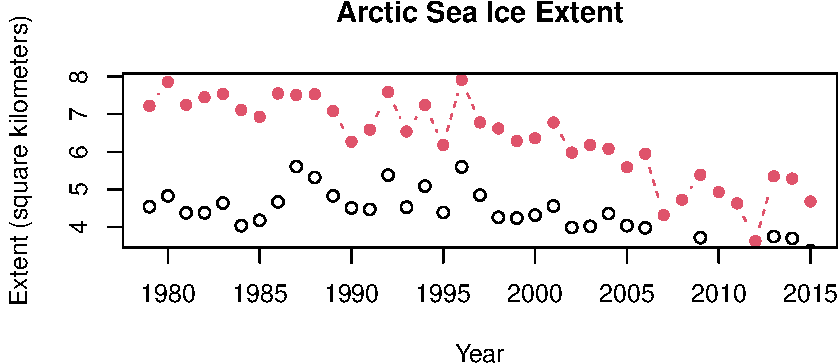
\includegraphics{compbio4all-book_files/figure-latex/unnamed-chunk-52-1.pdf}

\hypertarget{base-r-graphics}{%
\section{Base-R graphics}\label{base-r-graphics}}

When we use the \texttt{plot} command were using \textbf{Base R} graphics. As noted before there are several ways to make plots in R and you should be able to spot which one is which when looking at code. We'll cover some of the key features of Bare R graphics now. While different plotting methods have different commands and arguments, they all share a common feature: everything in a plot can be customized, and each element is customized with a command or arguement.

\hypertarget{type-of-points}{%
\subsection{Type of points}\label{type-of-points}}

\texttt{plot()} can draw dots or lines We make it use lines using the \texttt{type\ =\ "l"} argument (note that the l is in quotes)

\begin{Shaded}
\begin{Highlighting}[]
\FunctionTok{plot}\NormalTok{(Extent }\SpecialCharTok{\textasciitilde{}}\NormalTok{ Year, }\AttributeTok{type =} \StringTok{"l"}\NormalTok{, }\AttributeTok{data =}\NormalTok{ SeaIce)  }\CommentTok{\# Note: l in quotes}
\end{Highlighting}
\end{Shaded}

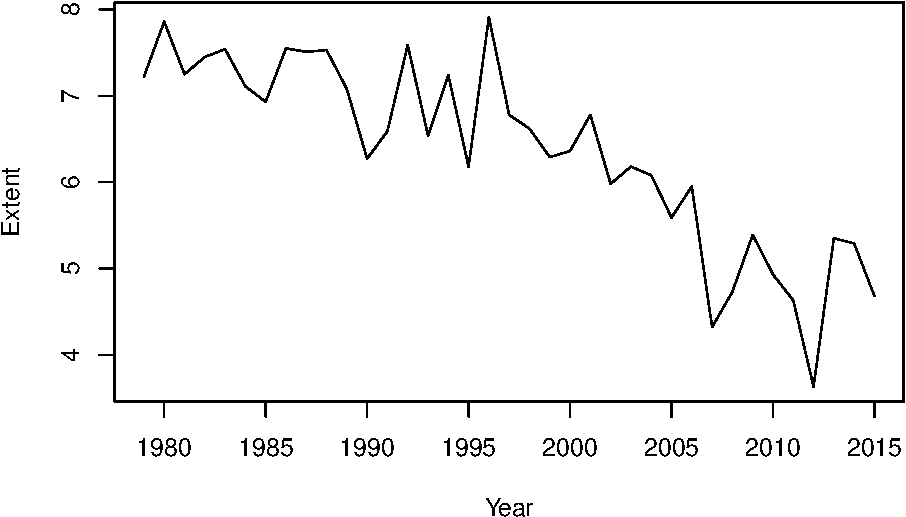
\includegraphics{compbio4all-book_files/figure-latex/unnamed-chunk-53-1.pdf}

As noted before, R doesn't mind if you split things on lines. To keep track of the things I''m doing to the plot I'll format things like this

\begin{Shaded}
\begin{Highlighting}[]
\FunctionTok{plot}\NormalTok{(Extent }\SpecialCharTok{\textasciitilde{}}\NormalTok{ Year,  }\CommentTok{\# relationship}
     \AttributeTok{type =} \StringTok{"l"}\NormalTok{,     }\CommentTok{\# type of plot; Note: l in quotes}
     \AttributeTok{data =}\NormalTok{ SeaIce)  }\CommentTok{\# data}
\end{Highlighting}
\end{Shaded}

As we did with the \texttt{lynx} data we can combine points and lines with \texttt{type\ =\ "b"}. (Do you recall what ``b'' stands for?)

\begin{Shaded}
\begin{Highlighting}[]
\FunctionTok{plot}\NormalTok{(Extent }\SpecialCharTok{\textasciitilde{}}\NormalTok{ Year,  }\CommentTok{\# relationship}
     \AttributeTok{type =} \StringTok{"b"}\NormalTok{,     }\CommentTok{\# type of plot; Note: b in quotes}
     \AttributeTok{data =}\NormalTok{ SeaIce)  }\CommentTok{\# data}
\end{Highlighting}
\end{Shaded}

We can adjust color with \texttt{col\ =\ ...}. Recall the this is just a number, not in quotes.

\begin{Shaded}
\begin{Highlighting}[]
\FunctionTok{plot}\NormalTok{(Extent }\SpecialCharTok{\textasciitilde{}}\NormalTok{ Year,  }\CommentTok{\# relationship}
     \AttributeTok{type =} \StringTok{"b"}\NormalTok{,     }\CommentTok{\# type of plot; Note: b in quotes}
     \AttributeTok{col =} \DecValTok{2}\NormalTok{,        }\CommentTok{\# color; no quotes}
     \AttributeTok{data =}\NormalTok{ SeaIce)  }\CommentTok{\# data}
\end{Highlighting}
\end{Shaded}

We can add a main title to with \texttt{main\ =\ ...}

\begin{Shaded}
\begin{Highlighting}[]
\FunctionTok{plot}\NormalTok{(Extent }\SpecialCharTok{\textasciitilde{}}\NormalTok{ Year,  }\CommentTok{\# relationship}
     \AttributeTok{type =} \StringTok{"b"}\NormalTok{,     }\CommentTok{\# type of plot; Note: b in quotes}
     \AttributeTok{col =} \DecValTok{2}\NormalTok{,        }\CommentTok{\# color; no quotes}
     \AttributeTok{main =} \StringTok{"Arctic Sea Ice Extent"}\NormalTok{, }\CommentTok{\# main title, in quotes}
     \AttributeTok{data =}\NormalTok{ SeaIce)  }\CommentTok{\# data}
\end{Highlighting}
\end{Shaded}

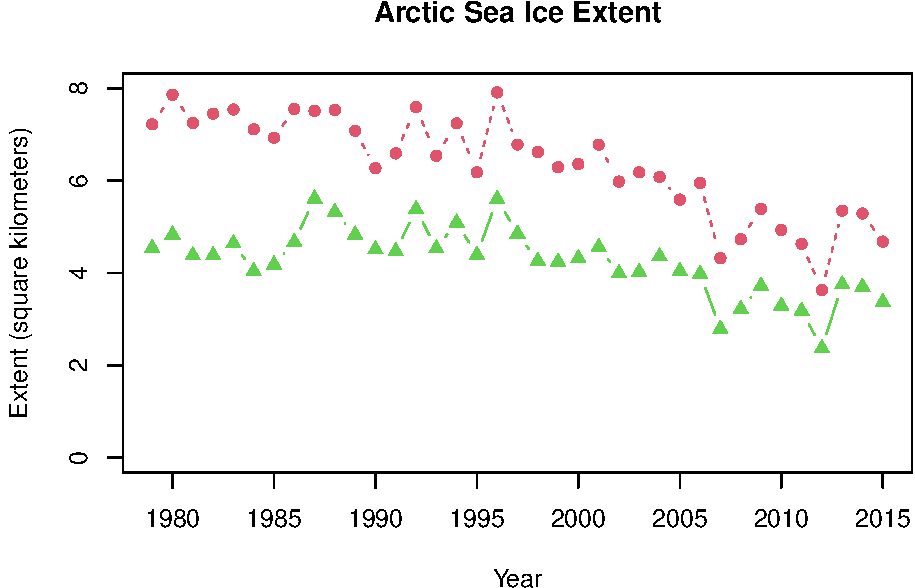
\includegraphics{compbio4all-book_files/figure-latex/unnamed-chunk-57-1.pdf}

Its always good to include your units. \texttt{Extent} and \texttt{Area} are in square kilometers. We can say specifically what we want for the y-axis label using \texttt{ylab\ =\ ...}

\begin{Shaded}
\begin{Highlighting}[]
\FunctionTok{plot}\NormalTok{(Extent }\SpecialCharTok{\textasciitilde{}}\NormalTok{ Year,  }\CommentTok{\# relationship}
     \AttributeTok{type =} \StringTok{"b"}\NormalTok{,     }\CommentTok{\# type of plot; Note: b in quotes}
     \AttributeTok{col =} \DecValTok{2}\NormalTok{,        }\CommentTok{\# color; no quotes}
     \AttributeTok{main =} \StringTok{"Arctic Sea Ice Extent"}\NormalTok{, }\CommentTok{\# main title, in quotes}
     \AttributeTok{ylab =} \StringTok{"Extent (square kilometers)"}\NormalTok{,}
     \AttributeTok{data =}\NormalTok{ SeaIce)  }\CommentTok{\# data}
\end{Highlighting}
\end{Shaded}

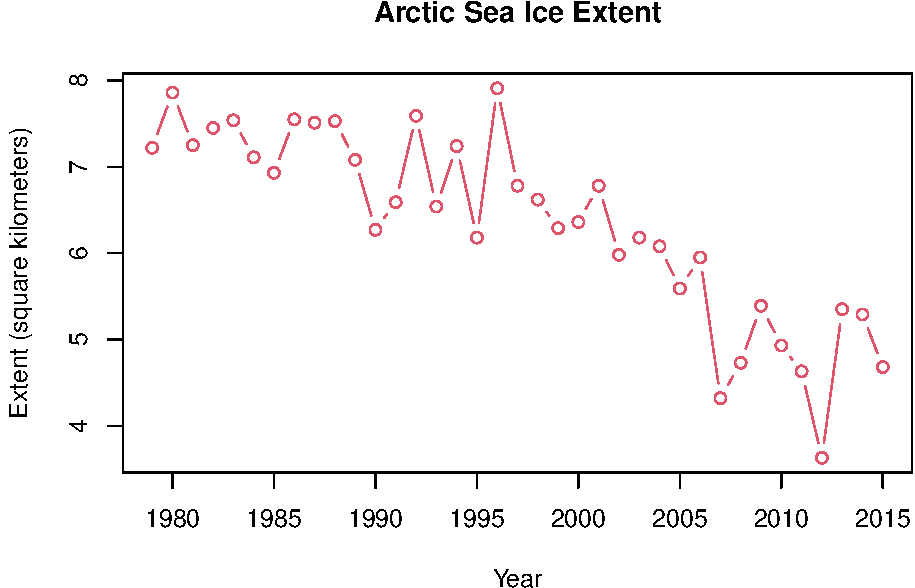
\includegraphics{compbio4all-book_files/figure-latex/unnamed-chunk-58-1.pdf}

We can change the appearance of the line using \texttt{lty\ =\ ...}, which stands for ``line type'':

\begin{Shaded}
\begin{Highlighting}[]
\FunctionTok{plot}\NormalTok{(Extent }\SpecialCharTok{\textasciitilde{}}\NormalTok{ Year,  }\CommentTok{\# relationship}
     \AttributeTok{type =} \StringTok{"b"}\NormalTok{,     }\CommentTok{\# type of plot; Note: b in quotes}
     \AttributeTok{col =} \DecValTok{2}\NormalTok{,        }\CommentTok{\# color; no quotes}
     \AttributeTok{main =} \StringTok{"Arctic Sea Ice Extent"}\NormalTok{, }\CommentTok{\# main title, in quotes}
     \AttributeTok{ylab =} \StringTok{"Extent (square kilometers)"}\NormalTok{,}
     \AttributeTok{lty =} \DecValTok{2}\NormalTok{,        }\CommentTok{\# line type; not quoted}
     \AttributeTok{data =}\NormalTok{ SeaIce)  }\CommentTok{\# data}
\end{Highlighting}
\end{Shaded}

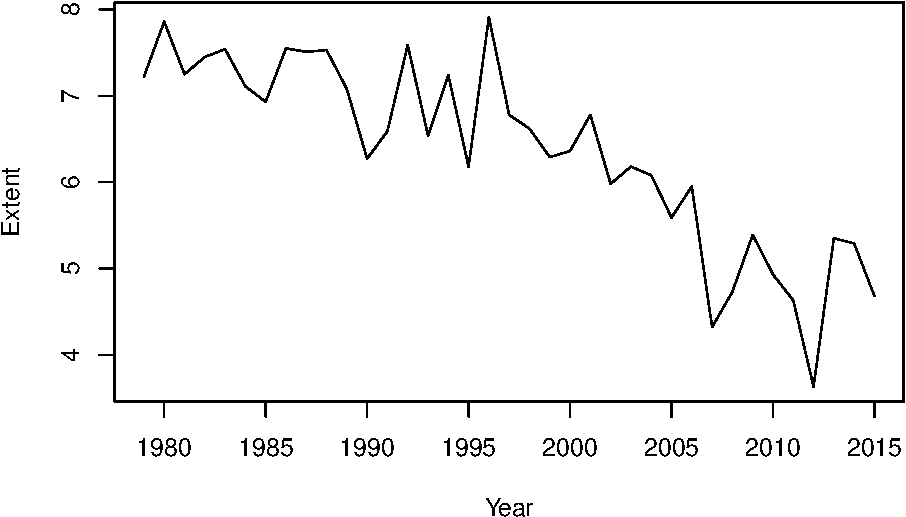
\includegraphics{compbio4all-book_files/figure-latex/unnamed-chunk-59-1.pdf}

I'm not a fan of the open circles for plotting points; we can change those too using the argument \texttt{pch\ =}.

\begin{Shaded}
\begin{Highlighting}[]
\FunctionTok{plot}\NormalTok{(Extent }\SpecialCharTok{\textasciitilde{}}\NormalTok{ Year,  }\CommentTok{\# relationship}
     \AttributeTok{type =} \StringTok{"b"}\NormalTok{,     }\CommentTok{\# type of plot; Note: b in quotes}
     \AttributeTok{col =} \DecValTok{2}\NormalTok{,        }\CommentTok{\# color; no quotes}
     \AttributeTok{main =} \StringTok{"Arctic Sea Ice Extent"}\NormalTok{, }\CommentTok{\# main title, in quotes}
     \AttributeTok{ylab =} \StringTok{"Extent (square kilometers)"}\NormalTok{,}
     \AttributeTok{lty =} \DecValTok{2}\NormalTok{,        }\CommentTok{\# line type; not quoted}
     \AttributeTok{pch =} \DecValTok{16}\NormalTok{,       }\CommentTok{\# point type; not quoted}
     \AttributeTok{data =}\NormalTok{ SeaIce)  }\CommentTok{\# data}
\end{Highlighting}
\end{Shaded}

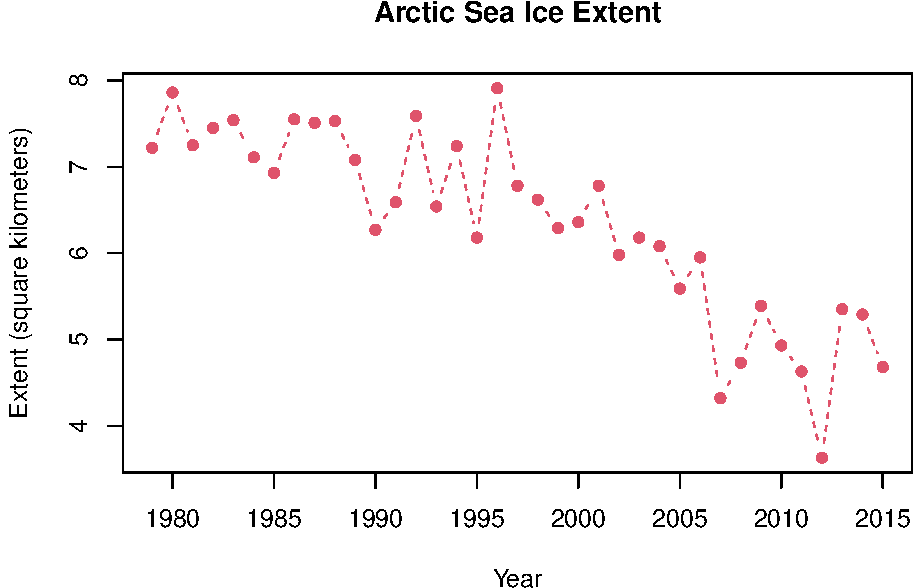
\includegraphics{compbio4all-book_files/figure-latex/unnamed-chunk-60-1.pdf}

\hypertarget{plotting-two-columns-of-data}{%
\subsection{Plotting two columns of data}\label{plotting-two-columns-of-data}}

Often we want to represent two distinct things on our graph. In spreadsheets these are called separate \textbf{series} of data. When making a \textbf{time series plot} like this one we can add a new column of data using a species command called \texttt{points()} which works very similar to \texttt{plot()}.

⚠️ \textbf{Note:} The \texttt{points()} command only works if its it precede by a statement from the \texttt{plot()} command ⚠️

\begin{Shaded}
\begin{Highlighting}[]
\CommentTok{\# Main plot: Extent}
\FunctionTok{plot}\NormalTok{(Extent }\SpecialCharTok{\textasciitilde{}}\NormalTok{ Year,  }\CommentTok{\# relationship}
     \AttributeTok{type =} \StringTok{"b"}\NormalTok{,     }\CommentTok{\# type of plot; Note: b in quotes}
     \AttributeTok{col =} \DecValTok{2}\NormalTok{,        }\CommentTok{\# color; no quotes}
     \AttributeTok{main =} \StringTok{"Arctic Sea Ice Extent"}\NormalTok{, }\CommentTok{\# main title, in quotes}
     \AttributeTok{ylab =} \StringTok{"Extent (square kilometers)"}\NormalTok{,}
     \AttributeTok{lty =} \DecValTok{2}\NormalTok{,        }\CommentTok{\# line type; not quoted}
     \AttributeTok{pch =} \DecValTok{16}\NormalTok{,       }\CommentTok{\# point type; not quoted}
     \AttributeTok{data =}\NormalTok{ SeaIce)  }\CommentTok{\# data}

\CommentTok{\# Second column of data: Area}
\FunctionTok{points}\NormalTok{(Area }\SpecialCharTok{\textasciitilde{}}\NormalTok{ Year, }\AttributeTok{data =}\NormalTok{ SeaIce)}
\end{Highlighting}
\end{Shaded}

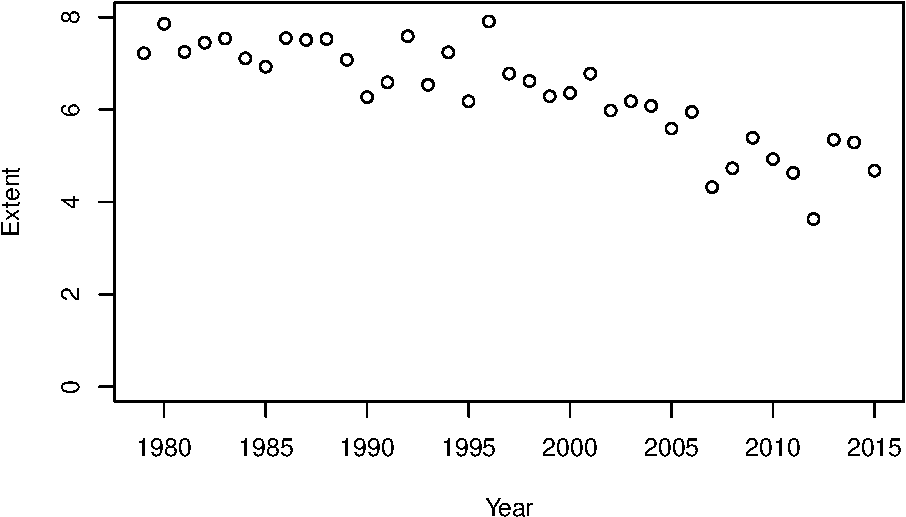
\includegraphics{compbio4all-book_files/figure-latex/unnamed-chunk-61-1.pdf}

I can now customize the sea ice \texttt{Area} part of the plot by add \textbf{arguments} to the \texttt{points()} statement.

\begin{Shaded}
\begin{Highlighting}[]
\CommentTok{\# Main plot: Extent}
\FunctionTok{plot}\NormalTok{(Extent }\SpecialCharTok{\textasciitilde{}}\NormalTok{ Year,  }\CommentTok{\# relationship}
     \AttributeTok{type =} \StringTok{"b"}\NormalTok{,     }\CommentTok{\# type of plot; Note: b in quotes}
     \AttributeTok{col =} \DecValTok{2}\NormalTok{,        }\CommentTok{\# color; no quotes}
     \AttributeTok{main =} \StringTok{"Arctic Sea Ice Extent"}\NormalTok{, }\CommentTok{\# main title, in quotes}
     \AttributeTok{ylab =} \StringTok{"Extent (square kilometers)"}\NormalTok{,}
     \AttributeTok{lty =} \DecValTok{2}\NormalTok{,        }\CommentTok{\# line type; not quoted}
     \AttributeTok{pch =} \DecValTok{16}\NormalTok{,       }\CommentTok{\# point type; not quoted}
     \AttributeTok{data =}\NormalTok{ SeaIce)  }\CommentTok{\# data}

\CommentTok{\# Second column of data: Area}
\FunctionTok{points}\NormalTok{(Area }\SpecialCharTok{\textasciitilde{}}\NormalTok{ Year,}
       \AttributeTok{type =} \StringTok{"b"}\NormalTok{,}
       \AttributeTok{col =} \DecValTok{3}\NormalTok{,}
       \AttributeTok{pch =} \DecValTok{17}\NormalTok{,}
       \AttributeTok{data =}\NormalTok{ SeaIce)}
\end{Highlighting}
\end{Shaded}

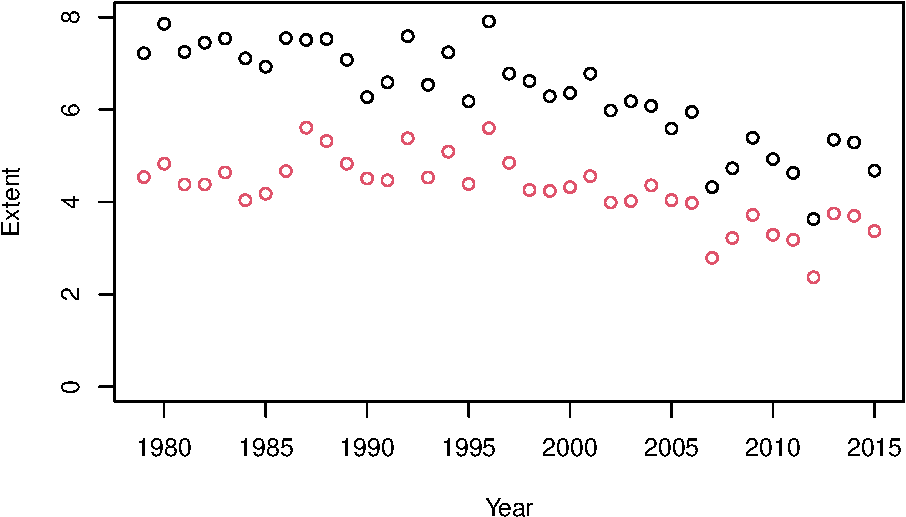
\includegraphics{compbio4all-book_files/figure-latex/unnamed-chunk-62-1.pdf}

❓ There's a problem with my graph though - can you spot it? It only really becomes apparent when you connect the dots with a line. ❓

\hypertarget{changing-the-range-of-a-plot-axis}{%
\subsection{Changing the range of a plot axis}\label{changing-the-range-of-a-plot-axis}}

Let's go back to our original plot and forget about all the fancy arguments and adding \texttt{points()} for a little bit. The problem with the last graph we made is that some points are not showing - if you look in the lower right-hand part points around 2006-2008 and 2011-2013 are not showing up because the y-axis stops around 3.5. We can fix this by adding a new argument which sets the limits of the y-axis: \texttt{ylim\ =\ ...}. To do this correctly, we have to introduce a new function: \texttt{c()}. This is actually one of the most common functions in R. In the \texttt{c()} we need to tell R the lower and upper limits we want for the y-axis. Let's do 0 and 8, which will be coded as \texttt{c(0,8)}.

So, to set the y-axis limits we do this:

\begin{Shaded}
\begin{Highlighting}[]
\FunctionTok{plot}\NormalTok{(Extent }\SpecialCharTok{\textasciitilde{}}\NormalTok{ Year,  }
     \AttributeTok{ylim =} \FunctionTok{c}\NormalTok{(}\DecValTok{0}\NormalTok{,}\DecValTok{8}\NormalTok{), }\CommentTok{\# the c(...) fucntion to set limits}
     \AttributeTok{data =}\NormalTok{ SeaIce) }
\end{Highlighting}
\end{Shaded}

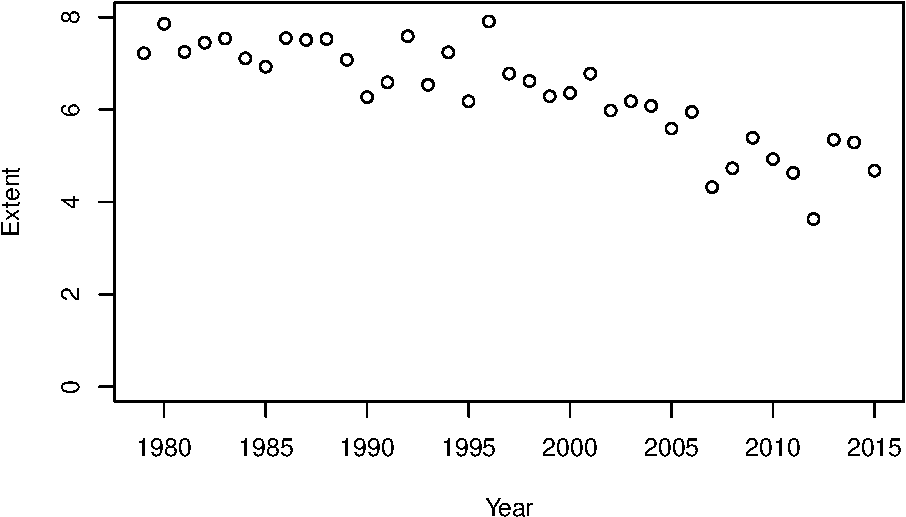
\includegraphics{compbio4all-book_files/figure-latex/unnamed-chunk-63-1.pdf}

Now we have a bunch more space at the bottom. We can add our \texttt{points()} back to see if this work:

\begin{Shaded}
\begin{Highlighting}[]
\FunctionTok{plot}\NormalTok{(Extent }\SpecialCharTok{\textasciitilde{}}\NormalTok{ Year,  }
     \AttributeTok{ylim =} \FunctionTok{c}\NormalTok{(}\DecValTok{0}\NormalTok{,}\DecValTok{8}\NormalTok{), }\CommentTok{\# the c(...) fucntion to set limits}
     \AttributeTok{data =}\NormalTok{ SeaIce) }
\FunctionTok{points}\NormalTok{(Area }\SpecialCharTok{\textasciitilde{}}\NormalTok{ Year,}
      \AttributeTok{data =}\NormalTok{ SeaIce,}
      \AttributeTok{col =} \DecValTok{2}\NormalTok{)}
\end{Highlighting}
\end{Shaded}

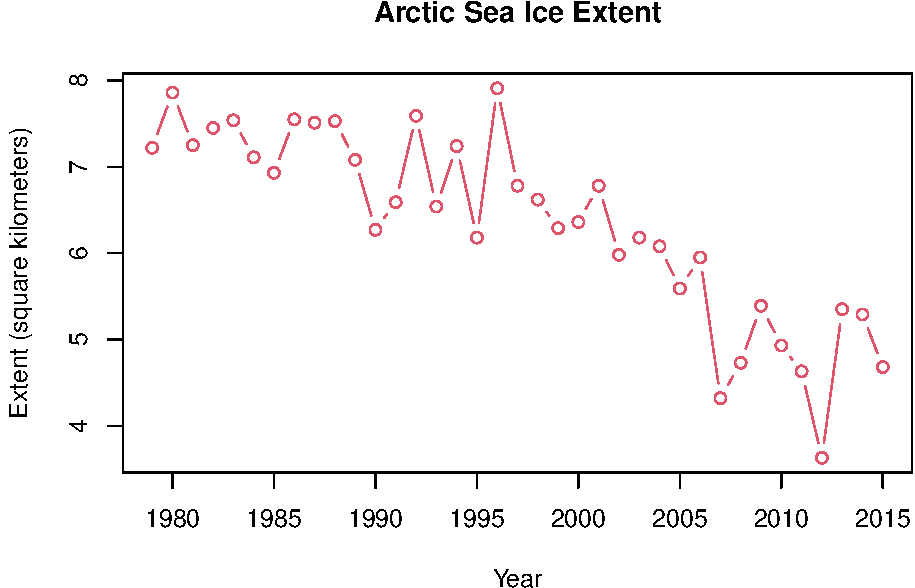
\includegraphics{compbio4all-book_files/figure-latex/unnamed-chunk-64-1.pdf}

⚠️ \textbf{Note:} \texttt{ylim\ =\ ...} only goes in \texttt{plot()}, not \texttt{points()}. \texttt{View()} ⚠️

Let's re-make our fancy plots now with \texttt{ylim\ =\ ...} set.

\begin{Shaded}
\begin{Highlighting}[]
\CommentTok{\# Main plot: Extent}
\FunctionTok{plot}\NormalTok{(Extent }\SpecialCharTok{\textasciitilde{}}\NormalTok{ Year,  }
     \AttributeTok{type =} \StringTok{"b"}\NormalTok{,     }
     \AttributeTok{col =} \DecValTok{2}\NormalTok{,       }
     \AttributeTok{main =} \StringTok{"Arctic Sea Ice Extent"}\NormalTok{, }
     \AttributeTok{ylab =} \StringTok{"Extent (square kilometers)"}\NormalTok{,}
     \AttributeTok{lty =} \DecValTok{2}\NormalTok{,        }
     \AttributeTok{pch =} \DecValTok{16}\NormalTok{,       }
     \AttributeTok{ylim =} \FunctionTok{c}\NormalTok{(}\DecValTok{0}\NormalTok{,}\DecValTok{8}\NormalTok{), }\CommentTok{\# \textless{}\#\textless{}== y{-}axis limits}
     \AttributeTok{data =}\NormalTok{ SeaIce)  }

\CommentTok{\# Second column of data: Area}
\FunctionTok{points}\NormalTok{(Area }\SpecialCharTok{\textasciitilde{}}\NormalTok{ Year,}
       \AttributeTok{type =} \StringTok{"b"}\NormalTok{,}
       \AttributeTok{col =} \DecValTok{3}\NormalTok{,}
       \AttributeTok{pch =} \DecValTok{17}\NormalTok{,}
       \AttributeTok{data =}\NormalTok{ SeaIce)}
\end{Highlighting}
\end{Shaded}

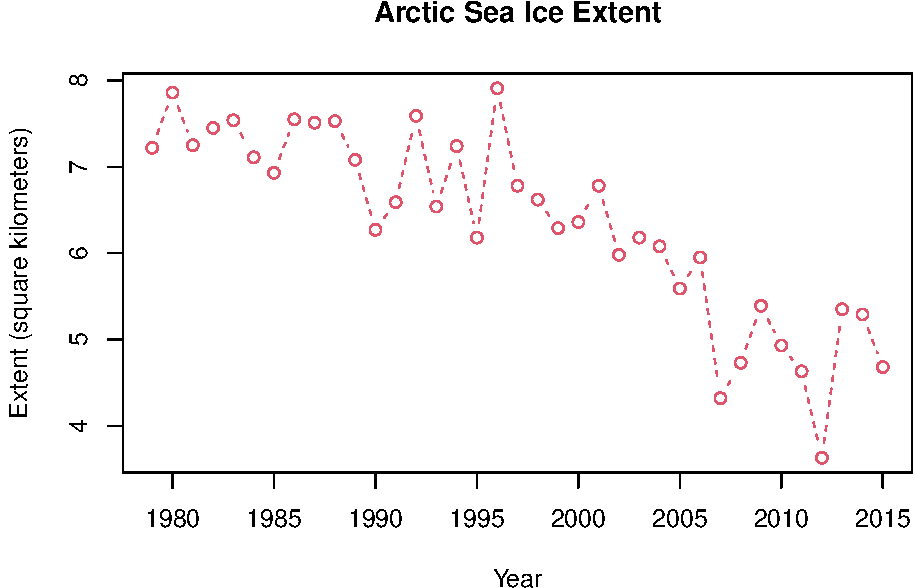
\includegraphics{compbio4all-book_files/figure-latex/unnamed-chunk-65-1.pdf}

\hypertarget{you-try-it}{%
\section{You try it}\label{you-try-it}}

\hypertarget{fixer-uppers}{%
\subsection{Fixer-uppers}\label{fixer-uppers}}

Fix the code below so it works

\begin{Shaded}
\begin{Highlighting}[]
\FunctionTok{plot}\NormalTok{(Extent , Year,  }
     \AttributeTok{data =}\NormalTok{ SeaIce)  }
\end{Highlighting}
\end{Shaded}

Fix the code below so it works

\begin{Shaded}
\begin{Highlighting}[]
\FunctionTok{plot}\NormalTok{(Extent }\SpecialCharTok{\textasciitilde{}}\NormalTok{ Year,  }\CommentTok{\# relationship}
     \AttributeTok{type =}\NormalTok{ b,     }\CommentTok{\# type of plot; Note: b in quotes}
     \AttributeTok{col =} \StringTok{"2"}\NormalTok{,        }\CommentTok{\# color; no quotes}
     \AttributeTok{data =}\NormalTok{ SeaIce)  }\CommentTok{\# data}
\end{Highlighting}
\end{Shaded}

\hypertarget{intermediate}{%
\subsection{Intermediate}\label{intermediate}}

Make a plot with \texttt{Area} on the x-axis and \texttt{Extent} on the y-axis.

\begin{Shaded}
\begin{Highlighting}[]
\DocumentationTok{\#\# Write the code below}
\end{Highlighting}
\end{Shaded}

\hypertarget{advanced}{%
\subsection{Advanced}\label{advanced}}

Based on the code above, make a plot of the SeaIce data where \texttt{Area} appears within the \texttt{plot()} statement, and \texttt{Extent} is in \texttt{points()}.

\begin{Shaded}
\begin{Highlighting}[]
\CommentTok{\# Write the code below: }
\end{Highlighting}
\end{Shaded}

\hypertarget{build-your-own-dataframe-part-i-vectors}{%
\chapter{Build your own dataframe part I: Vectors}\label{build-your-own-dataframe-part-i-vectors}}

\hypertarget{dataframes-are-a-type-of-data-structure}{%
\section{Dataframes are a type of data structure}\label{dataframes-are-a-type-of-data-structure}}

For small datasets its often useful to build your own dataframes. Dataframes are \textbf{objects} in R; in particular they are a type of \textbf{data structure}. ``Data structure'' is just a fancy way of saying ``holding or organizing data.''

We'll work with the \texttt{SeaIce} data again.

\begin{Shaded}
\begin{Highlighting}[]
\FunctionTok{library}\NormalTok{(Stat2Data)}
\FunctionTok{data}\NormalTok{(}\StringTok{"SeaIce"}\NormalTok{)}
\end{Highlighting}
\end{Shaded}

If we're curious about what kind of data is in an object we can use the \texttt{class()} command to see how is is classified.. Generally the first thing R spits out is the most important.

\begin{Shaded}
\begin{Highlighting}[]
\FunctionTok{class}\NormalTok{(SeaIce)}
\end{Highlighting}
\end{Shaded}

\begin{verbatim}
## [1] "data.frame"
\end{verbatim}

We see that \texttt{SeaIce\ is\ a}data.frame`.

A related command is \texttt{is()}

\begin{Shaded}
\begin{Highlighting}[]
\FunctionTok{is}\NormalTok{(SeaIce)}
\end{Highlighting}
\end{Shaded}

\begin{verbatim}
## [1] "data.frame" "list"       "oldClass"   "vector"
\end{verbatim}

This command is more \textbf{verbose} and tells of several things, the most relevant of which is that \texttt{SeaIce} is a dataframe.

The \texttt{SeaIce} dataframe has several columns. We can pull up their names using the \texttt{names()} command.

\begin{Shaded}
\begin{Highlighting}[]
\FunctionTok{names}\NormalTok{(SeaIce)}
\end{Highlighting}
\end{Shaded}

\begin{verbatim}
## [1] "Year"   "Extent" "Area"   "t"
\end{verbatim}

There are times when we may want to examine just a single column. We can isolate a single column using a species notation which uses a dollar sign. To get the \texttt{Extent} column we do this

\begin{Shaded}
\begin{Highlighting}[]
\NormalTok{SeaIce}\SpecialCharTok{$}\NormalTok{Extent}
\end{Highlighting}
\end{Shaded}

\begin{verbatim}
##  [1] 7.22 7.86 7.25 7.45 7.54 7.11 6.93 7.55 7.51 7.53 7.08 6.27 6.59 7.59 6.54
## [16] 7.24 6.18 7.91 6.78 6.62 6.29 6.36 6.78 5.98 6.18 6.08 5.59 5.95 4.32 4.73
## [31] 5.39 4.93 4.63 3.63 5.35 5.29 4.68
\end{verbatim}

\hypertarget{dataframes-are-made-from-vectors}{%
\section{Dataframes are made from vectors}\label{dataframes-are-made-from-vectors}}

Running this we get just a stream of numbers. In R, such a stream of numbers is called a \textbf{vector}. Like dataframes, vectors are a type of data structure. We can check this with \texttt{is()}

\begin{Shaded}
\begin{Highlighting}[]
\FunctionTok{is}\NormalTok{(SeaIce}\SpecialCharTok{$}\NormalTok{Extent)}
\end{Highlighting}
\end{Shaded}

\begin{verbatim}
## [1] "numeric" "vector"
\end{verbatim}

The first result is \texttt{numeric}, which indicates that there are numbers in this vector; the second result is vector.

All columns in a dataframe are are vectors:

\begin{Shaded}
\begin{Highlighting}[]
\FunctionTok{is}\NormalTok{(SeaIce}\SpecialCharTok{$}\NormalTok{Year)}
\end{Highlighting}
\end{Shaded}

\begin{verbatim}
## [1] "integer"             "double"              "numeric"            
## [4] "vector"              "data.frameRowLabels"
\end{verbatim}

\begin{Shaded}
\begin{Highlighting}[]
\FunctionTok{is}\NormalTok{(SeaIce}\SpecialCharTok{$}\NormalTok{Area)}
\end{Highlighting}
\end{Shaded}

\begin{verbatim}
## [1] "numeric" "vector"
\end{verbatim}

\hypertarget{make-your-own-vectors}{%
\section{Make your own vectors}\label{make-your-own-vectors}}

We can make our own vectors using the \texttt{c()} command. (\texttt{c()} does MANY things in R, so we'll see it a lot).

Here is some more recent data on the Canda Lynx from 1984 to 2002 (Poole 2003, Table 3):

\begin{Shaded}
\begin{Highlighting}[]
\FunctionTok{c}\NormalTok{(}\DecValTok{13445}\NormalTok{, }\DecValTok{8625}\NormalTok{, }\DecValTok{6853}\NormalTok{, }\DecValTok{6953}\NormalTok{, }\DecValTok{6574}\NormalTok{,}
  \DecValTok{8265}\NormalTok{, }\DecValTok{9977}\NormalTok{, }\DecValTok{7579}\NormalTok{, }\DecValTok{11542}\NormalTok{, }\DecValTok{7180}\NormalTok{,}
  \DecValTok{4713}\NormalTok{, }\DecValTok{4907}\NormalTok{, }\DecValTok{2819}\NormalTok{, }\DecValTok{5171}\NormalTok{, }\DecValTok{6873}\NormalTok{, }
  \DecValTok{6148}\NormalTok{, }\DecValTok{8573}\NormalTok{, }\DecValTok{9361}\NormalTok{, }\DecValTok{11226}\NormalTok{)}
\end{Highlighting}
\end{Shaded}

\begin{verbatim}
##  [1] 13445  8625  6853  6953  6574  8265  9977  7579 11542  7180  4713  4907
## [13]  2819  5171  6873  6148  8573  9361 11226
\end{verbatim}

We can save this to an R object using a very species function in R called the \textbf{assigment operator}

\begin{Shaded}
\begin{Highlighting}[]
\NormalTok{lynx.ca }\OtherTok{\textless{}{-}} \FunctionTok{c}\NormalTok{(}\DecValTok{13445}\NormalTok{, }\DecValTok{8625}\NormalTok{, }\DecValTok{6853}\NormalTok{, }\DecValTok{6953}\NormalTok{, }\DecValTok{6574}\NormalTok{,}
  \DecValTok{8265}\NormalTok{, }\DecValTok{9977}\NormalTok{, }\DecValTok{7579}\NormalTok{, }\DecValTok{11542}\NormalTok{, }\DecValTok{7180}\NormalTok{,}
  \DecValTok{4713}\NormalTok{, }\DecValTok{4907}\NormalTok{, }\DecValTok{2819}\NormalTok{, }\DecValTok{5171}\NormalTok{, }\DecValTok{6873}\NormalTok{, }
  \DecValTok{6148}\NormalTok{, }\DecValTok{8573}\NormalTok{, }\DecValTok{9361}\NormalTok{, }\DecValTok{11226}\NormalTok{)}
\end{Highlighting}
\end{Shaded}

We've now made a brand new object in R called \texttt{lynx.ca}. We can see what it is by just typing its name in the console\ldots{}

\begin{Shaded}
\begin{Highlighting}[]
\NormalTok{lynx.ca}
\end{Highlighting}
\end{Shaded}

\begin{verbatim}
##  [1] 13445  8625  6853  6953  6574  8265  9977  7579 11542  7180  4713  4907
## [13]  2819  5171  6873  6148  8573  9361 11226
\end{verbatim}

\ldots and confirming what it is with \texttt{is()} and \texttt{class()}

\begin{Shaded}
\begin{Highlighting}[]
\FunctionTok{is}\NormalTok{(lynx.ca)}
\end{Highlighting}
\end{Shaded}

\begin{verbatim}
## [1] "numeric" "vector"
\end{verbatim}

\begin{Shaded}
\begin{Highlighting}[]
\FunctionTok{class}\NormalTok{(lynx.ca)}
\end{Highlighting}
\end{Shaded}

\begin{verbatim}
## [1] "numeric"
\end{verbatim}

The data are from 1984 to 2002. We can make a \texttt{year} vector like this

\begin{Shaded}
\begin{Highlighting}[]
\NormalTok{year }\OtherTok{\textless{}{-}} \FunctionTok{c}\NormalTok{(}\DecValTok{1984}\NormalTok{, }\DecValTok{1985}\NormalTok{, }\DecValTok{1986}\NormalTok{, }\DecValTok{1987}\NormalTok{,}
          \DecValTok{1988}\NormalTok{, }\DecValTok{1989}\NormalTok{, }\DecValTok{1990}\NormalTok{, }\DecValTok{1991}\NormalTok{, }\DecValTok{1992}\NormalTok{, }
          \DecValTok{1993}\NormalTok{, }\DecValTok{1994}\NormalTok{, }\DecValTok{1995}\NormalTok{, }\DecValTok{1996}\NormalTok{, }\DecValTok{1997}\NormalTok{,}
          \DecValTok{1998}\NormalTok{, }\DecValTok{1999}\NormalTok{, }\DecValTok{2000}\NormalTok{, }\DecValTok{2001}\NormalTok{, }\DecValTok{2002}\NormalTok{)}
\end{Highlighting}
\end{Shaded}

Its rather tedious to do that, so R has a trick. If we want a sequence of numbers we can use the \texttt{seq()} command, which has the arguments \texttt{from\ =...} and \texttt{to\ =\ ...}.

\begin{Shaded}
\begin{Highlighting}[]
\NormalTok{year }\OtherTok{\textless{}{-}} \FunctionTok{seq}\NormalTok{(}\AttributeTok{from =} \DecValTok{1984}\NormalTok{, }\AttributeTok{to =} \DecValTok{2002}\NormalTok{)}
\end{Highlighting}
\end{Shaded}

\hypertarget{checking-the-length-of-vectors}{%
\section{Checking the length of vectors}\label{checking-the-length-of-vectors}}

Typing in data directly into R is errorprone and whenever we do it we should check our work carefully. A first check should be that we entered in all the numbers; we can do this by getting R to tell us the length of the vector. Can you guess what the command is called?

\begin{Shaded}
\begin{Highlighting}[]
\FunctionTok{length}\NormalTok{(lynx.ca)}
\end{Highlighting}
\end{Shaded}

\begin{verbatim}
## [1] 19
\end{verbatim}

Let's check that our year vector is the same length

\begin{Shaded}
\begin{Highlighting}[]
\FunctionTok{length}\NormalTok{(year)}
\end{Highlighting}
\end{Shaded}

\begin{verbatim}
## [1] 19
\end{verbatim}

\hypertarget{another-example}{%
\section{Another example}\label{another-example}}

Another famous example

Howlett and Majerus. 1987. The understanding of industrial melanism in the peppered moth (\emph{Biston betularia}) .(Lepidoptera: Geometridae). 30: 31-44.

Table 2

\begin{Shaded}
\begin{Highlighting}[]
\NormalTok{year.ne }\OtherTok{\textless{}{-}} \FunctionTok{c}\NormalTok{(}\DecValTok{1954}\NormalTok{, }\DecValTok{1961}\NormalTok{, }\DecValTok{1970}\NormalTok{, }\DecValTok{1975}\NormalTok{, }\DecValTok{1981}\NormalTok{, }\DecValTok{1982}\NormalTok{, }\DecValTok{1983}\NormalTok{, }\DecValTok{1984}\NormalTok{, }\DecValTok{1985}\NormalTok{)}

\NormalTok{moths.ne }\OtherTok{\textless{}{-}} \FunctionTok{c}\NormalTok{(}\FloatTok{92.95}\NormalTok{, }\FloatTok{94.78}\NormalTok{, }\DecValTok{75}\NormalTok{, }\FloatTok{64.7}\NormalTok{, }\FloatTok{45.9}\NormalTok{, }\DecValTok{50}\NormalTok{, }\FloatTok{42.9}\NormalTok{, }\FloatTok{42.1}\NormalTok{, }\FloatTok{39.6}\NormalTok{)}
\end{Highlighting}
\end{Shaded}

(Raw data is slightly more complicated, but this works)

\begin{Shaded}
\begin{Highlighting}[]
\FunctionTok{length}\NormalTok{(year.ne)}
\end{Highlighting}
\end{Shaded}

\begin{verbatim}
## [1] 9
\end{verbatim}

\begin{Shaded}
\begin{Highlighting}[]
\FunctionTok{length}\NormalTok{(moths.ne)}
\end{Highlighting}
\end{Shaded}

\begin{verbatim}
## [1] 9
\end{verbatim}

\begin{Shaded}
\begin{Highlighting}[]
\NormalTok{moths }\OtherTok{\textless{}{-}} \FunctionTok{data.frame}\NormalTok{(year.ne,}
\NormalTok{                    moths.ne)}
\end{Highlighting}
\end{Shaded}

\begin{Shaded}
\begin{Highlighting}[]
\FunctionTok{plot}\NormalTok{(moths.ne }\SpecialCharTok{\textasciitilde{}}\NormalTok{ year.ne, }\AttributeTok{data =}\NormalTok{ moths)}
\end{Highlighting}
\end{Shaded}

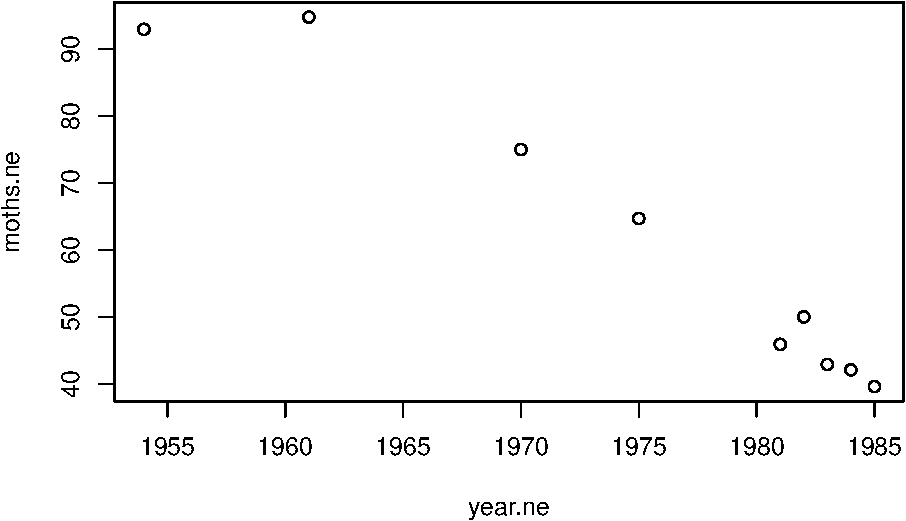
\includegraphics{compbio4all-book_files/figure-latex/unnamed-chunk-88-1.pdf}

Not how R doesn't need extra space for the years where there are no data

\hypertarget{try-it-yourself}{%
\section{Try it yourself}\label{try-it-yourself}}

The original lynx data that comes with R spans the year 1821--1934. Make a sequence of numbers called year.lynx using the \texttt{seq()} command.

\begin{Shaded}
\begin{Highlighting}[]
\DecValTok{1957}\SpecialCharTok{:}\DecValTok{1964}
\end{Highlighting}
\end{Shaded}

\begin{verbatim}
## [1] 1957 1958 1959 1960 1961 1962 1963 1964
\end{verbatim}

There was a hypothesis that sunspot number and/or size impact lynx populations. R has a dataset called sunspots that runs from 1749 to 1983. Make a vector called year year.sunspot using the \texttt{seq()} command.

\begin{Shaded}
\begin{Highlighting}[]
\DecValTok{1749}\SpecialCharTok{:}\DecValTok{1983}
\end{Highlighting}
\end{Shaded}

\begin{verbatim}
##   [1] 1749 1750 1751 1752 1753 1754 1755 1756 1757 1758 1759 1760 1761 1762 1763
##  [16] 1764 1765 1766 1767 1768 1769 1770 1771 1772 1773 1774 1775 1776 1777 1778
##  [31] 1779 1780 1781 1782 1783 1784 1785 1786 1787 1788 1789 1790 1791 1792 1793
##  [46] 1794 1795 1796 1797 1798 1799 1800 1801 1802 1803 1804 1805 1806 1807 1808
##  [61] 1809 1810 1811 1812 1813 1814 1815 1816 1817 1818 1819 1820 1821 1822 1823
##  [76] 1824 1825 1826 1827 1828 1829 1830 1831 1832 1833 1834 1835 1836 1837 1838
##  [91] 1839 1840 1841 1842 1843 1844 1845 1846 1847 1848 1849 1850 1851 1852 1853
## [106] 1854 1855 1856 1857 1858 1859 1860 1861 1862 1863 1864 1865 1866 1867 1868
## [121] 1869 1870 1871 1872 1873 1874 1875 1876 1877 1878 1879 1880 1881 1882 1883
## [136] 1884 1885 1886 1887 1888 1889 1890 1891 1892 1893 1894 1895 1896 1897 1898
## [151] 1899 1900 1901 1902 1903 1904 1905 1906 1907 1908 1909 1910 1911 1912 1913
## [166] 1914 1915 1916 1917 1918 1919 1920 1921 1922 1923 1924 1925 1926 1927 1928
## [181] 1929 1930 1931 1932 1933 1934 1935 1936 1937 1938 1939 1940 1941 1942 1943
## [196] 1944 1945 1946 1947 1948 1949 1950 1951 1952 1953 1954 1955 1956 1957 1958
## [211] 1959 1960 1961 1962 1963 1964 1965 1966 1967 1968 1969 1970 1971 1972 1973
## [226] 1974 1975 1976 1977 1978 1979 1980 1981 1982 1983
\end{verbatim}

\hypertarget{a-complicate-dataframe-to-make}{%
\section{A complicate dataframe to make}\label{a-complicate-dataframe-to-make}}

\hypertarget{build-the-dataframe}{%
\section{Build the dataframe}\label{build-the-dataframe}}

This code makes all of the columns and makes a dataframe

\begin{Shaded}
\begin{Highlighting}[]
\NormalTok{aa        }\OtherTok{\textless{}{-}}\FunctionTok{c}\NormalTok{(}\StringTok{\textquotesingle{}A\textquotesingle{}}\NormalTok{,}\StringTok{\textquotesingle{}C\textquotesingle{}}\NormalTok{,}\StringTok{\textquotesingle{}D\textquotesingle{}}\NormalTok{,}\StringTok{\textquotesingle{}E\textquotesingle{}}\NormalTok{,}\StringTok{\textquotesingle{}F\textquotesingle{}}\NormalTok{,}\StringTok{\textquotesingle{}G\textquotesingle{}}\NormalTok{,}\StringTok{\textquotesingle{}H\textquotesingle{}}\NormalTok{,}\StringTok{\textquotesingle{}I\textquotesingle{}}\NormalTok{,}\StringTok{\textquotesingle{}K\textquotesingle{}}\NormalTok{,}\StringTok{\textquotesingle{}L\textquotesingle{}}\NormalTok{,}\StringTok{\textquotesingle{}M\textquotesingle{}}\NormalTok{,}\StringTok{\textquotesingle{}N\textquotesingle{}}\NormalTok{,}\StringTok{\textquotesingle{}P\textquotesingle{}}\NormalTok{,}\StringTok{\textquotesingle{}Q\textquotesingle{}}\NormalTok{,}\StringTok{\textquotesingle{}R\textquotesingle{}}\NormalTok{,}\StringTok{\textquotesingle{}S\textquotesingle{}}\NormalTok{,}\StringTok{\textquotesingle{}T\textquotesingle{}}\NormalTok{,}\StringTok{\textquotesingle{}V\textquotesingle{}}\NormalTok{,}\StringTok{\textquotesingle{}W\textquotesingle{}}\NormalTok{,}\StringTok{\textquotesingle{}Y\textquotesingle{}}\NormalTok{)}
\NormalTok{MW.da     }\OtherTok{\textless{}{-}}\FunctionTok{c}\NormalTok{(}\DecValTok{89}\NormalTok{,}\DecValTok{121}\NormalTok{,}\DecValTok{133}\NormalTok{,}\DecValTok{146}\NormalTok{,}\DecValTok{165}\NormalTok{,}\DecValTok{75}\NormalTok{,}\DecValTok{155}\NormalTok{,}\DecValTok{131}\NormalTok{,}\DecValTok{146}\NormalTok{,}\DecValTok{131}\NormalTok{,}\DecValTok{149}\NormalTok{,}\DecValTok{132}\NormalTok{,}\DecValTok{115}\NormalTok{,}\DecValTok{147}\NormalTok{,}\DecValTok{174}\NormalTok{,}\DecValTok{105}\NormalTok{,}\DecValTok{119}\NormalTok{,}\DecValTok{117}\NormalTok{,}\DecValTok{204}\NormalTok{,}\DecValTok{181}\NormalTok{)}
\NormalTok{volume    }\OtherTok{\textless{}{-}}\FunctionTok{c}\NormalTok{(}\DecValTok{67}\NormalTok{,}\DecValTok{86}\NormalTok{,}\DecValTok{91}\NormalTok{,}\DecValTok{109}\NormalTok{,}\DecValTok{135}\NormalTok{,}\DecValTok{48}\NormalTok{,}\DecValTok{118}\NormalTok{,}\DecValTok{124}\NormalTok{,}\DecValTok{135}\NormalTok{,}\DecValTok{124}\NormalTok{,}\DecValTok{124}\NormalTok{,}\DecValTok{96}\NormalTok{,}\DecValTok{90}\NormalTok{,}
              \DecValTok{114}\NormalTok{,}\DecValTok{148}\NormalTok{,}\DecValTok{73}\NormalTok{,}\DecValTok{93}\NormalTok{,}\DecValTok{105}\NormalTok{,}\DecValTok{163}\NormalTok{,}\DecValTok{141}\NormalTok{)}
\NormalTok{bulkiness }\OtherTok{\textless{}{-}}\FunctionTok{c}\NormalTok{(}\FloatTok{11.5}\NormalTok{,}\FloatTok{13.46}\NormalTok{,}\FloatTok{11.68}\NormalTok{,}\FloatTok{13.57}\NormalTok{,}\FloatTok{19.8}\NormalTok{,}\FloatTok{3.4}\NormalTok{,}\FloatTok{13.69}\NormalTok{,}\FloatTok{21.4}\NormalTok{,}
              \FloatTok{15.71}\NormalTok{,}\FloatTok{21.4}\NormalTok{,}\FloatTok{16.25}\NormalTok{,}\FloatTok{12.28}\NormalTok{,}\FloatTok{17.43}\NormalTok{,}
              \FloatTok{14.45}\NormalTok{,}\FloatTok{14.28}\NormalTok{,}\FloatTok{9.47}\NormalTok{,}\FloatTok{15.77}\NormalTok{,}\FloatTok{21.57}\NormalTok{,}\FloatTok{21.67}\NormalTok{,}\FloatTok{18.03}\NormalTok{)}
\NormalTok{polarity  }\OtherTok{\textless{}{-}}\FunctionTok{c}\NormalTok{(}\DecValTok{0}\NormalTok{,}\FloatTok{1.48}\NormalTok{,}\FloatTok{49.7}\NormalTok{,}\FloatTok{49.9}\NormalTok{,}\FloatTok{0.35}\NormalTok{,}\DecValTok{0}\NormalTok{,}\FloatTok{51.6}\NormalTok{,}\FloatTok{0.13}\NormalTok{,}\FloatTok{49.5}\NormalTok{,}\FloatTok{0.13}\NormalTok{,}
              \FloatTok{1.43}\NormalTok{,}\FloatTok{3.38}\NormalTok{,}\FloatTok{1.58}\NormalTok{,}\FloatTok{3.53}\NormalTok{,}\DecValTok{52}\NormalTok{,}\FloatTok{1.67}\NormalTok{,}\FloatTok{1.66}\NormalTok{,}\FloatTok{0.13}\NormalTok{,}\FloatTok{2.1}\NormalTok{,}\FloatTok{1.61}\NormalTok{)}
\NormalTok{isoelectric.pt }\OtherTok{\textless{}{-}}\FunctionTok{c}\NormalTok{(}\DecValTok{6}\NormalTok{,}\FloatTok{5.07}\NormalTok{,}\FloatTok{2.77}\NormalTok{,}\FloatTok{3.22}\NormalTok{,}\FloatTok{5.48}\NormalTok{,}\FloatTok{5.97}\NormalTok{,}\FloatTok{7.59}\NormalTok{,}\FloatTok{6.02}\NormalTok{,}\FloatTok{9.74}\NormalTok{,}\FloatTok{5.98}\NormalTok{,}
                   \FloatTok{5.74}\NormalTok{,}\FloatTok{5.41}\NormalTok{,}\FloatTok{6.3}\NormalTok{,}\FloatTok{5.65}\NormalTok{,}\FloatTok{10.76}\NormalTok{,}\FloatTok{5.68}\NormalTok{,}\FloatTok{6.16}\NormalTok{,}\FloatTok{5.96}\NormalTok{,}\FloatTok{5.89}\NormalTok{,}\FloatTok{5.66}\NormalTok{)}
\NormalTok{hydrophobe}\FloatTok{.34} \OtherTok{\textless{}{-}}\FunctionTok{c}\NormalTok{(}\FloatTok{1.8}\NormalTok{,}\FloatTok{2.5}\NormalTok{,}\SpecialCharTok{{-}}\FloatTok{3.5}\NormalTok{,}\SpecialCharTok{{-}}\FloatTok{3.5}\NormalTok{,}\FloatTok{2.8}\NormalTok{,}\SpecialCharTok{{-}}\FloatTok{0.4}\NormalTok{,}\SpecialCharTok{{-}}\FloatTok{3.2}\NormalTok{,}\FloatTok{4.5}\NormalTok{,}\SpecialCharTok{{-}}\FloatTok{3.9}\NormalTok{,}\FloatTok{3.8}\NormalTok{,}\FloatTok{1.9}\NormalTok{,}
                  \SpecialCharTok{{-}}\FloatTok{3.5}\NormalTok{,}\SpecialCharTok{{-}}\FloatTok{1.6}\NormalTok{,}\SpecialCharTok{{-}}\FloatTok{3.5}\NormalTok{,}\SpecialCharTok{{-}}\FloatTok{4.5}\NormalTok{,}\SpecialCharTok{{-}}\FloatTok{0.8}\NormalTok{,}\SpecialCharTok{{-}}\FloatTok{0.7}\NormalTok{,}\FloatTok{4.2}\NormalTok{,}\SpecialCharTok{{-}}\FloatTok{0.9}\NormalTok{,}\SpecialCharTok{{-}}\FloatTok{1.3}\NormalTok{)}
\NormalTok{hydrophobe}\FloatTok{.35} \OtherTok{\textless{}{-}}\FunctionTok{c}\NormalTok{(}\FloatTok{1.6}\NormalTok{,}\DecValTok{2}\NormalTok{,}\SpecialCharTok{{-}}\FloatTok{9.2}\NormalTok{,}\SpecialCharTok{{-}}\FloatTok{8.2}\NormalTok{,}\FloatTok{3.7}\NormalTok{,}\DecValTok{1}\NormalTok{,}\SpecialCharTok{{-}}\DecValTok{3}\NormalTok{,}\FloatTok{3.1}\NormalTok{,}\SpecialCharTok{{-}}\FloatTok{8.8}\NormalTok{,}\FloatTok{2.8}\NormalTok{,}\FloatTok{3.4}\NormalTok{,}\SpecialCharTok{{-}}\FloatTok{4.8}\NormalTok{,}
                  \SpecialCharTok{{-}}\FloatTok{0.2}\NormalTok{,}\SpecialCharTok{{-}}\FloatTok{4.1}\NormalTok{,}\SpecialCharTok{{-}}\FloatTok{12.3}\NormalTok{,}\FloatTok{0.6}\NormalTok{,}\FloatTok{1.2}\NormalTok{,}\FloatTok{2.6}\NormalTok{,}\FloatTok{1.9}\NormalTok{,}\SpecialCharTok{{-}}\FloatTok{0.7}\NormalTok{)}
\NormalTok{saaH2O       }\OtherTok{\textless{}{-}}\FunctionTok{c}\NormalTok{(}\DecValTok{113}\NormalTok{,}\DecValTok{140}\NormalTok{,}\DecValTok{151}\NormalTok{,}\DecValTok{183}\NormalTok{,}\DecValTok{218}\NormalTok{,}\DecValTok{85}\NormalTok{,}\DecValTok{194}\NormalTok{,}\DecValTok{182}\NormalTok{,}\DecValTok{211}\NormalTok{,}\DecValTok{180}\NormalTok{,}\DecValTok{204}\NormalTok{,}\DecValTok{158}\NormalTok{,}
                 \DecValTok{143}\NormalTok{,}\DecValTok{189}\NormalTok{,}\DecValTok{241}\NormalTok{,}\DecValTok{122}\NormalTok{,}\DecValTok{146}\NormalTok{,}\DecValTok{160}\NormalTok{,}\DecValTok{259}\NormalTok{,}\DecValTok{229}\NormalTok{)}
\NormalTok{faal.fold    }\OtherTok{\textless{}{-}}\FunctionTok{c}\NormalTok{(}\FloatTok{0.74}\NormalTok{,}\FloatTok{0.91}\NormalTok{,}\FloatTok{0.62}\NormalTok{,}\FloatTok{0.62}\NormalTok{,}\FloatTok{0.88}\NormalTok{,}\FloatTok{0.72}\NormalTok{,}\FloatTok{0.78}\NormalTok{,}\FloatTok{0.88}\NormalTok{,}\FloatTok{0.52}\NormalTok{,}
                 \FloatTok{0.85}\NormalTok{,}\FloatTok{0.85}\NormalTok{,}\FloatTok{0.63}\NormalTok{,}\FloatTok{0.64}\NormalTok{,}\FloatTok{0.62}\NormalTok{,}\FloatTok{0.64}\NormalTok{,}\FloatTok{0.66}\NormalTok{,}\FloatTok{0.7}\NormalTok{,}\FloatTok{0.86}\NormalTok{,}\FloatTok{0.85}\NormalTok{,}\FloatTok{0.76}\NormalTok{)}
\NormalTok{polar.req    }\OtherTok{\textless{}{-}}\FunctionTok{c}\NormalTok{(}\DecValTok{7}\NormalTok{,}\FloatTok{4.8}\NormalTok{,}\DecValTok{13}\NormalTok{,}\FloatTok{12.5}\NormalTok{,}\DecValTok{5}\NormalTok{,}\FloatTok{7.9}\NormalTok{,}\FloatTok{8.4}\NormalTok{,}\FloatTok{4.9}\NormalTok{,}\FloatTok{10.1}\NormalTok{,}\FloatTok{4.9}\NormalTok{,}\FloatTok{5.3}\NormalTok{,}\DecValTok{10}\NormalTok{,}
                 \FloatTok{6.6}\NormalTok{,}\FloatTok{8.6}\NormalTok{,}\FloatTok{9.1}\NormalTok{,}\FloatTok{7.5}\NormalTok{,}\FloatTok{6.6}\NormalTok{,}\FloatTok{5.6}\NormalTok{,}\FloatTok{5.2}\NormalTok{,}\FloatTok{5.4}\NormalTok{)}
\NormalTok{freq        }\OtherTok{\textless{}{-}}\FunctionTok{c}\NormalTok{(}\FloatTok{7.8}\NormalTok{,}\FloatTok{1.1}\NormalTok{,}\FloatTok{5.19}\NormalTok{,}\FloatTok{6.72}\NormalTok{,}\FloatTok{4.39}\NormalTok{,}\FloatTok{6.77}\NormalTok{,}\FloatTok{2.03}\NormalTok{,}\FloatTok{6.95}\NormalTok{,}\FloatTok{6.32}\NormalTok{,}
                \FloatTok{10.15}\NormalTok{,}\FloatTok{2.28}\NormalTok{,}\FloatTok{4.37}\NormalTok{,}\FloatTok{4.26}\NormalTok{,}\FloatTok{3.45}\NormalTok{,}\FloatTok{5.23}\NormalTok{,}\FloatTok{6.46}\NormalTok{,}\FloatTok{5.12}\NormalTok{,}\FloatTok{7.01}\NormalTok{,}\FloatTok{1.09}\NormalTok{,}\FloatTok{3.3}\NormalTok{)}
\NormalTok{charge}\OtherTok{\textless{}{-}}\FunctionTok{c}\NormalTok{(}\StringTok{\textquotesingle{}un\textquotesingle{}}\NormalTok{,}\StringTok{\textquotesingle{}un\textquotesingle{}}\NormalTok{,}\StringTok{\textquotesingle{}neg\textquotesingle{}}\NormalTok{,}\StringTok{\textquotesingle{}neg\textquotesingle{}}\NormalTok{,}\StringTok{\textquotesingle{}un\textquotesingle{}}\NormalTok{,}\StringTok{\textquotesingle{}un\textquotesingle{}}\NormalTok{,}\StringTok{\textquotesingle{}pos\textquotesingle{}}\NormalTok{,}\StringTok{\textquotesingle{}un\textquotesingle{}}\NormalTok{,}\StringTok{\textquotesingle{}pos\textquotesingle{}}\NormalTok{,}
          \StringTok{\textquotesingle{}un\textquotesingle{}}\NormalTok{,}\StringTok{\textquotesingle{}un\textquotesingle{}}\NormalTok{,}\StringTok{\textquotesingle{}un\textquotesingle{}}\NormalTok{,}\StringTok{\textquotesingle{}un\textquotesingle{}}\NormalTok{,}\StringTok{\textquotesingle{}un\textquotesingle{}}\NormalTok{,}\StringTok{\textquotesingle{}pos\textquotesingle{}}\NormalTok{,}\StringTok{\textquotesingle{}un\textquotesingle{}}\NormalTok{,}\StringTok{\textquotesingle{}un\textquotesingle{}}\NormalTok{,}\StringTok{\textquotesingle{}un\textquotesingle{}}\NormalTok{,}\StringTok{\textquotesingle{}un\textquotesingle{}}\NormalTok{,}\StringTok{\textquotesingle{}un\textquotesingle{}}\NormalTok{)}
\NormalTok{hydropathy}\OtherTok{\textless{}{-}}\FunctionTok{c}\NormalTok{(}\StringTok{\textquotesingle{}hydrophobic\textquotesingle{}}\NormalTok{,}\StringTok{\textquotesingle{}hydrophobic\textquotesingle{}}\NormalTok{,}\StringTok{\textquotesingle{}hydrophilic\textquotesingle{}}\NormalTok{,}\StringTok{\textquotesingle{}hydrophilic\textquotesingle{}}\NormalTok{,}\StringTok{\textquotesingle{}hydrophobic\textquotesingle{}}\NormalTok{,}\StringTok{\textquotesingle{}neutral\textquotesingle{}}\NormalTok{,}\StringTok{\textquotesingle{}neutral\textquotesingle{}}\NormalTok{,}\StringTok{\textquotesingle{}hydrophobic\textquotesingle{}}\NormalTok{,}\StringTok{\textquotesingle{}hydrophilic\textquotesingle{}}\NormalTok{,}\StringTok{\textquotesingle{}hydrophobic\textquotesingle{}}\NormalTok{,}\StringTok{\textquotesingle{}hydrophobic\textquotesingle{}}\NormalTok{,}\StringTok{\textquotesingle{}hydrophilic\textquotesingle{}}\NormalTok{,}\StringTok{\textquotesingle{}neutral\textquotesingle{}}\NormalTok{,}\StringTok{\textquotesingle{}hydrophilic\textquotesingle{}}\NormalTok{,}\StringTok{\textquotesingle{}hydrophilic\textquotesingle{}}\NormalTok{,}\StringTok{\textquotesingle{}neutral\textquotesingle{}}\NormalTok{,}\StringTok{\textquotesingle{}neutral\textquotesingle{}}\NormalTok{,}
              \StringTok{\textquotesingle{}hydrophobic\textquotesingle{}}\NormalTok{,}\StringTok{\textquotesingle{}hydrophobic\textquotesingle{}}\NormalTok{,}\StringTok{\textquotesingle{}neutral\textquotesingle{}}\NormalTok{)}
\NormalTok{volume.cat}\OtherTok{\textless{}{-}}\FunctionTok{c}\NormalTok{(}\StringTok{\textquotesingle{}verysmall\textquotesingle{}}\NormalTok{,}\StringTok{\textquotesingle{}small\textquotesingle{}}\NormalTok{,}\StringTok{\textquotesingle{}small\textquotesingle{}}\NormalTok{,}\StringTok{\textquotesingle{}medium\textquotesingle{}}\NormalTok{,}
              \StringTok{\textquotesingle{}verylarge\textquotesingle{}}\NormalTok{,}\StringTok{\textquotesingle{}verysmall\textquotesingle{}}\NormalTok{,}\StringTok{\textquotesingle{}medium\textquotesingle{}}\NormalTok{,}\StringTok{\textquotesingle{}large\textquotesingle{}}\NormalTok{,}\StringTok{\textquotesingle{}large\textquotesingle{}}\NormalTok{,}
              \StringTok{\textquotesingle{}large\textquotesingle{}}\NormalTok{,}\StringTok{\textquotesingle{}large\textquotesingle{}}\NormalTok{,}\StringTok{\textquotesingle{}small\textquotesingle{}}\NormalTok{,}\StringTok{\textquotesingle{}small\textquotesingle{}}\NormalTok{,}\StringTok{\textquotesingle{}medium\textquotesingle{}}\NormalTok{,}\StringTok{\textquotesingle{}large\textquotesingle{}}\NormalTok{,}\StringTok{\textquotesingle{}verysmall\textquotesingle{}}\NormalTok{,}\StringTok{\textquotesingle{}small\textquotesingle{}}\NormalTok{,}\StringTok{\textquotesingle{}medium\textquotesingle{}}\NormalTok{,}\StringTok{\textquotesingle{}verylarge\textquotesingle{}}\NormalTok{,}\StringTok{\textquotesingle{}verylarge\textquotesingle{}}\NormalTok{)}
\NormalTok{polarity.cat}\OtherTok{\textless{}{-}}\FunctionTok{c}\NormalTok{(}\StringTok{\textquotesingle{}nonpolar\textquotesingle{}}\NormalTok{,}\StringTok{\textquotesingle{}nonpolar\textquotesingle{}}\NormalTok{,}\StringTok{\textquotesingle{}polar\textquotesingle{}}\NormalTok{,}\StringTok{\textquotesingle{}polar\textquotesingle{}}\NormalTok{,}
                \StringTok{\textquotesingle{}nonpolar\textquotesingle{}}\NormalTok{,}\StringTok{\textquotesingle{}nonpolar\textquotesingle{}}\NormalTok{,}\StringTok{\textquotesingle{}polar\textquotesingle{}}\NormalTok{,}\StringTok{\textquotesingle{}nonpolar\textquotesingle{}}\NormalTok{,}
                \StringTok{\textquotesingle{}polar\textquotesingle{}}\NormalTok{,}\StringTok{\textquotesingle{}nonpolar\textquotesingle{}}\NormalTok{,}\StringTok{\textquotesingle{}nonpolar\textquotesingle{}}\NormalTok{,}\StringTok{\textquotesingle{}polar\textquotesingle{}}\NormalTok{,}\StringTok{\textquotesingle{}nonpolar\textquotesingle{}}\NormalTok{,}\StringTok{\textquotesingle{}polar\textquotesingle{}}\NormalTok{,}
                \StringTok{\textquotesingle{}polar\textquotesingle{}}\NormalTok{,}\StringTok{\textquotesingle{}polar\textquotesingle{}}\NormalTok{,}\StringTok{\textquotesingle{}polar\textquotesingle{}}\NormalTok{,}\StringTok{\textquotesingle{}nonpolar\textquotesingle{}}\NormalTok{,}\StringTok{\textquotesingle{}nonpolar\textquotesingle{}}\NormalTok{,}\StringTok{\textquotesingle{}polar\textquotesingle{}}\NormalTok{)}
\NormalTok{chemical}\OtherTok{\textless{}{-}}\FunctionTok{c}\NormalTok{(}\StringTok{\textquotesingle{}aliphatic\textquotesingle{}}\NormalTok{,}\StringTok{\textquotesingle{}sulfur\textquotesingle{}}\NormalTok{,}\StringTok{\textquotesingle{}acidic\textquotesingle{}}\NormalTok{,}\StringTok{\textquotesingle{}acidic\textquotesingle{}}\NormalTok{,}\StringTok{\textquotesingle{}aromatic\textquotesingle{}}\NormalTok{,}
            \StringTok{\textquotesingle{}aliphatic\textquotesingle{}}\NormalTok{,}\StringTok{\textquotesingle{}basic\textquotesingle{}}\NormalTok{,}\StringTok{\textquotesingle{}aliphatic\textquotesingle{}}\NormalTok{,}\StringTok{\textquotesingle{}basic\textquotesingle{}}\NormalTok{,}\StringTok{\textquotesingle{}aliphatic\textquotesingle{}}\NormalTok{,}\StringTok{\textquotesingle{}sulfur\textquotesingle{}}\NormalTok{,}
            \StringTok{\textquotesingle{}amide\textquotesingle{}}\NormalTok{,}\StringTok{\textquotesingle{}aliphatic\textquotesingle{}}\NormalTok{,}\StringTok{\textquotesingle{}amide\textquotesingle{}}\NormalTok{,}\StringTok{\textquotesingle{}basic\textquotesingle{}}\NormalTok{,}\StringTok{\textquotesingle{}hydroxyl\textquotesingle{}}\NormalTok{,}\StringTok{\textquotesingle{}hydroxyl\textquotesingle{}}\NormalTok{,}
            \StringTok{\textquotesingle{}aliphatic\textquotesingle{}}\NormalTok{,}\StringTok{\textquotesingle{}aromatic\textquotesingle{}}\NormalTok{,}\StringTok{\textquotesingle{}aromatic\textquotesingle{}}\NormalTok{)}

\NormalTok{aa\_dat }\OtherTok{\textless{}{-}} \FunctionTok{data.frame}\NormalTok{(aa,MW.da,volume,bulkiness,}
\NormalTok{polarity,isoelectric.pt,hydrophobe}\FloatTok{.34}\NormalTok{,hydrophobe}\FloatTok{.35}\NormalTok{,}
\NormalTok{saaH2O,faal.fold, polar.req,freq,charge,hydropathy,volume.cat,polarity.cat,chemical)}
\end{Highlighting}
\end{Shaded}

Try plotting one numeric variable against another.

\hypertarget{factors}{%
\subsection{Factors}\label{factors}}

The amino acid data contains both \textbf{numeric} data and vectors of words that represent categories or groups of similar amino acids. When the dataframe first is created R doesn't do anything with it. For example, if we look at a numeric variable, we get this summary information

\begin{Shaded}
\begin{Highlighting}[]
\FunctionTok{summary}\NormalTok{(aa\_dat}\SpecialCharTok{$}\NormalTok{MW.da)}
\end{Highlighting}
\end{Shaded}

\begin{verbatim}
##    Min. 1st Qu.  Median    Mean 3rd Qu.    Max. 
##    75.0   118.5   132.5   136.8   150.5   204.0
\end{verbatim}

If we do the same summary command on a column of text we get this

\begin{Shaded}
\begin{Highlighting}[]
\FunctionTok{summary}\NormalTok{(aa\_dat}\SpecialCharTok{$}\NormalTok{hydropathy)}
\end{Highlighting}
\end{Shaded}

\begin{verbatim}
##    Length     Class      Mode 
##        20 character character
\end{verbatim}

We can help R make sense of this columns usin the command factor().

\begin{Shaded}
\begin{Highlighting}[]
\NormalTok{aa\_dat}\SpecialCharTok{$}\NormalTok{hydropathy }\OtherTok{\textless{}{-}} \FunctionTok{factor}\NormalTok{(aa\_dat}\SpecialCharTok{$}\NormalTok{hydropathy)}
\end{Highlighting}
\end{Shaded}

Note that on the right is the command

\begin{Shaded}
\begin{Highlighting}[]
\FunctionTok{factor}\NormalTok{(aa\_dat}\SpecialCharTok{$}\NormalTok{hydropathy)}
\end{Highlighting}
\end{Shaded}

and on the left we are assigning the output of this function back onto the original column, thus telling R that the words in this column represent group or categories.
(The term ``factor'' comes from statistics and isn't very helpful about what's going on.)

\begin{Shaded}
\begin{Highlighting}[]
\FunctionTok{summary}\NormalTok{(aa\_dat}\SpecialCharTok{$}\NormalTok{hydropathy)}
\end{Highlighting}
\end{Shaded}

\begin{verbatim}
## hydrophilic hydrophobic     neutral 
##           6           8           6
\end{verbatim}

Note that if I do this

\begin{Shaded}
\begin{Highlighting}[]
\NormalTok{aa\_dat }\OtherTok{\textless{}{-}} \FunctionTok{factor}\NormalTok{(aa\_dat}\SpecialCharTok{$}\NormalTok{hydropathy)}
\end{Highlighting}
\end{Shaded}

I \textbf{overwrite} the entire aa\_dat dataframe object with the data of just the aa\_dat\$hydropathy column.

\hypertarget{references}{%
\section{References}\label{references}}

Poole, Kim G. 2003. A review of the Canada Lynx, \emph{Lynx canadensis} ,in Canada. Canadian {[}Field-Naturalist 117: 360-376.{[}(\url{https://www.canadianfieldnaturalist.ca/index.php/cfn/article/view/738}){]} DOI: \url{https://doi.org/10.22621/cfn.v117i3.738}

\hypertarget{build-your-own-dataframe}{%
\chapter{Build your own dataframe}\label{build-your-own-dataframe}}

Build a dataframe from the data below and practice making plots

Number of lynx

\begin{Shaded}
\begin{Highlighting}[]
\NormalTok{lynx.ca }\OtherTok{\textless{}{-}} \FunctionTok{c}\NormalTok{(}\DecValTok{13445}\NormalTok{, }\DecValTok{8625}\NormalTok{, }\DecValTok{6853}\NormalTok{, }\DecValTok{6953}\NormalTok{, }\DecValTok{6574}\NormalTok{,}
  \DecValTok{8265}\NormalTok{, }\DecValTok{9977}\NormalTok{, }\DecValTok{7579}\NormalTok{, }\DecValTok{11542}\NormalTok{, }\DecValTok{7180}\NormalTok{,}
  \DecValTok{4713}\NormalTok{, }\DecValTok{4907}\NormalTok{, }\DecValTok{2819}\NormalTok{, }\DecValTok{5171}\NormalTok{, }\DecValTok{6873}\NormalTok{, }
  \DecValTok{6148}\NormalTok{, }\DecValTok{8573}\NormalTok{, }\DecValTok{9361}\NormalTok{, }\DecValTok{11226}\NormalTok{)}
\end{Highlighting}
\end{Shaded}

Year of study

\begin{Shaded}
\begin{Highlighting}[]
\NormalTok{year }\OtherTok{\textless{}{-}} \FunctionTok{c}\NormalTok{(}\DecValTok{1984}\NormalTok{, }\DecValTok{1985}\NormalTok{, }\DecValTok{1986}\NormalTok{, }\DecValTok{1987}\NormalTok{,}
          \DecValTok{1988}\NormalTok{, }\DecValTok{1989}\NormalTok{, }\DecValTok{1990}\NormalTok{, }\DecValTok{1991}\NormalTok{, }\DecValTok{1992}\NormalTok{, }
          \DecValTok{1993}\NormalTok{, }\DecValTok{1994}\NormalTok{, }\DecValTok{1995}\NormalTok{, }\DecValTok{1996}\NormalTok{, }\DecValTok{1997}\NormalTok{,}
          \DecValTok{1998}\NormalTok{, }\DecValTok{1999}\NormalTok{, }\DecValTok{2000}\NormalTok{, }\DecValTok{2001}\NormalTok{, }\DecValTok{2002}\NormalTok{)}
\end{Highlighting}
\end{Shaded}

Make the dataframe.

\begin{Shaded}
\begin{Highlighting}[]
\NormalTok{lynx.new }\OtherTok{\textless{}{-}} \FunctionTok{data.frame}\NormalTok{(lynx.ca,}
\NormalTok{                    year)}
\end{Highlighting}
\end{Shaded}

Build a basic plot

\begin{Shaded}
\begin{Highlighting}[]
\FunctionTok{plot}\NormalTok{(lynx.ca }\SpecialCharTok{\textasciitilde{}}\NormalTok{ year, }\AttributeTok{data =}\NormalTok{ lynx.new)}
\end{Highlighting}
\end{Shaded}

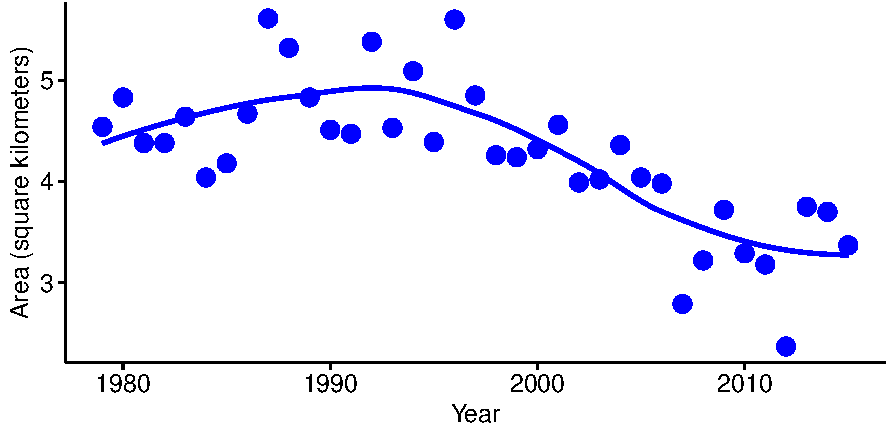
\includegraphics{compbio4all-book_files/figure-latex/unnamed-chunk-101-1.pdf}

As in the lynx dataset that comes with R, we see wild swings in abundance over short periods of time.

\hypertarget{your-turn-1}{%
\section{Your turn}\label{your-turn-1}}

Make this plot nice. Change the x axis label, y axis label, give it a main title, etc.

\hypertarget{references-1}{%
\section{References}\label{references-1}}

Poole, Kim G. 2003. A review of the Canada Lynx, \emph{Lynx canadensis} ,in Canada. Canadian {[}Field-Naturalist 117: 360-376.{[}(\url{https://www.canadianfieldnaturalist.ca/index.php/cfn/article/view/738}){]} DOI: \url{https://doi.org/10.22621/cfn.v117i3.738}

  \bibliography{book.bib,packages.bib}

\end{document}
